\documentclass[twoside]{book}

% Packages required by doxygen
\usepackage{calc}
\usepackage{doxygen}
\usepackage{graphicx}
\usepackage[utf8]{inputenc}
\usepackage{makeidx}
\usepackage{multicol}
\usepackage{multirow}
\usepackage{textcomp}
\usepackage[table]{xcolor}

% Font selection
\usepackage[T1]{fontenc}
\usepackage{mathptmx}
\usepackage[scaled=.90]{helvet}
\usepackage{courier}
\usepackage{amssymb}
\usepackage{sectsty}
\renewcommand{\familydefault}{\sfdefault}
\allsectionsfont{%
  \fontseries{bc}\selectfont%
  \color{darkgray}%
}
\renewcommand{\DoxyLabelFont}{%
  \fontseries{bc}\selectfont%
  \color{darkgray}%
}

% Page & text layout
\usepackage{geometry}
\geometry{%
  a4paper,%
  top=2.5cm,%
  bottom=2.5cm,%
  left=2.5cm,%
  right=2.5cm%
}
\tolerance=750
\hfuzz=15pt
\hbadness=750
\setlength{\emergencystretch}{15pt}
\setlength{\parindent}{0cm}
\setlength{\parskip}{0.2cm}
\makeatletter
\renewcommand{\paragraph}{%
  \@startsection{paragraph}{4}{0ex}{-1.0ex}{1.0ex}{%
    \normalfont\normalsize\bfseries\SS@parafont%
  }%
}
\renewcommand{\subparagraph}{%
  \@startsection{subparagraph}{5}{0ex}{-1.0ex}{1.0ex}{%
    \normalfont\normalsize\bfseries\SS@subparafont%
  }%
}
\makeatother

% Headers & footers
\usepackage{fancyhdr}
\pagestyle{fancyplain}
\fancyhead[LE]{\fancyplain{}{\bfseries\thepage}}
\fancyhead[CE]{\fancyplain{}{}}
\fancyhead[RE]{\fancyplain{}{\bfseries\leftmark}}
\fancyhead[LO]{\fancyplain{}{\bfseries\rightmark}}
\fancyhead[CO]{\fancyplain{}{}}
\fancyhead[RO]{\fancyplain{}{\bfseries\thepage}}
\fancyfoot[LE]{\fancyplain{}{}}
\fancyfoot[CE]{\fancyplain{}{}}
\fancyfoot[RE]{\fancyplain{}{\bfseries\scriptsize Generated on Tue Aug 26 2014 03\-:37\-:13 for 234\-Tree by Doxygen }}
\fancyfoot[LO]{\fancyplain{}{\bfseries\scriptsize Generated on Tue Aug 26 2014 03\-:37\-:13 for 234\-Tree by Doxygen }}
\fancyfoot[CO]{\fancyplain{}{}}
\fancyfoot[RO]{\fancyplain{}{}}
\renewcommand{\footrulewidth}{0.4pt}
\renewcommand{\chaptermark}[1]{%
  \markboth{#1}{}%
}
\renewcommand{\sectionmark}[1]{%
  \markright{\thesection\ #1}%
}

% Indices & bibliography
\usepackage{natbib}
\usepackage[titles]{tocloft}
\setcounter{tocdepth}{3}
\setcounter{secnumdepth}{5}
\makeindex

% Hyperlinks (required, but should be loaded last)
\usepackage{ifpdf}
\ifpdf
  \usepackage[pdftex,pagebackref=true]{hyperref}
\else
  \usepackage[ps2pdf,pagebackref=true]{hyperref}
\fi
\hypersetup{%
  colorlinks=true,%
  linkcolor=blue,%
  citecolor=blue,%
  unicode%
}

% Custom commands
\newcommand{\clearemptydoublepage}{%
  \newpage{\pagestyle{empty}\cleardoublepage}%
}


%===== C O N T E N T S =====

\begin{document}

% Titlepage & ToC
\hypersetup{pageanchor=false}
\pagenumbering{roman}
\begin{titlepage}
\vspace*{7cm}
\begin{center}%
{\Large 234\-Tree }\\
\vspace*{1cm}
{\large Generated by Doxygen 1.8.6}\\
\vspace*{0.5cm}
{\small Tue Aug 26 2014 03:37:13}\\
\end{center}
\end{titlepage}
\clearemptydoublepage
\tableofcontents
\clearemptydoublepage
\pagenumbering{arabic}
\hypersetup{pageanchor=true}

%--- Begin generated contents ---
\chapter{Main page}
\label{index}\hypertarget{index}{}\hypertarget{index_intro_sec}{}\section{Purpose}\label{index_intro_sec}
This is a project for the course Data Structures at the Computer Engineering and Informatics Department, University of Patras. The purpose of this project was to implement basic sorting and searching algorithms.\hypertarget{index_compile_sec}{}\section{Compiling}\label{index_compile_sec}
\begin{center} mkdir build \&\& cd build \&\& cmake .. \&\& make \&\& cd .. \end{center} \hypertarget{index_run_sec}{}\section{Running}\label{index_run_sec}
\begin{center} cd bin \&\& ./sort\-Nsearch \end{center} \hypertarget{index_dep_sec}{}\section{Dependancies (\-Debian based systems)}\label{index_dep_sec}
\begin{center} sudo apt-\/get install cmake (Minimum version 2.\-6 required) \end{center} \hypertarget{index_info_sec}{}\section{More information}\label{index_info_sec}
Contact\-: \href{mailto:b.papaspyros@gmail.com}{\tt b.\-papaspyros@gmail.\-com} or create an issue on the github page \href{https://github.com/bpapaspyros/DataStructures}{\tt https\-://github.\-com/bpapaspyros/\-Data\-Structures}

\begin{DoxyAuthor}{Author}
Vaios Papaspyros 
\end{DoxyAuthor}

\chapter{Class Index}
\section{Class List}
Here are the classes, structs, unions and interfaces with brief descriptions\-:\begin{DoxyCompactList}
\item\contentsline{section}{\hyperlink{class_graph_vis}{Graph\-Vis} \\*\hyperlink{class_graph_vis}{Graph\-Vis} Class }{\pageref{class_graph_vis}}{}
\item\contentsline{section}{\hyperlink{class_interface}{Interface} \\*\hyperlink{class_interface}{Interface} Class }{\pageref{class_interface}}{}
\item\contentsline{section}{\hyperlink{class_node}{Node} \\*\hyperlink{class_node}{Node} Class }{\pageref{class_node}}{}
\item\contentsline{section}{\hyperlink{class_tree}{Tree} \\*\hyperlink{class_tree}{Tree} Class }{\pageref{class_tree}}{}
\end{DoxyCompactList}

\chapter{File Index}
\section{File List}
Here is a list of all files with brief descriptions\-:\begin{DoxyCompactList}
\item\contentsline{section}{/home/baios/\-Coding/\-C++/\-Git\-Data\-Structures/\-Data\-Structures/234\-Tree/build/\-C\-Make\-Files/2.\-8.\-12.\-2/\-Compiler\-Id\-C/\hyperlink{_c_make_c_compiler_id_8c}{C\-Make\-C\-Compiler\-Id.\-c} }{\pageref{_c_make_c_compiler_id_8c}}{}
\item\contentsline{section}{/home/baios/\-Coding/\-C++/\-Git\-Data\-Structures/\-Data\-Structures/234\-Tree/build/\-C\-Make\-Files/2.\-8.\-12.\-2/\-Compiler\-Id\-C\-X\-X/\hyperlink{_c_make_c_x_x_compiler_id_8cpp}{C\-Make\-C\-X\-X\-Compiler\-Id.\-cpp} }{\pageref{_c_make_c_x_x_compiler_id_8cpp}}{}
\item\contentsline{section}{/home/baios/\-Coding/\-C++/\-Git\-Data\-Structures/\-Data\-Structures/234\-Tree/include/\hyperlink{_graph_vis_8h}{Graph\-Vis.\-h} }{\pageref{_graph_vis_8h}}{}
\item\contentsline{section}{/home/baios/\-Coding/\-C++/\-Git\-Data\-Structures/\-Data\-Structures/234\-Tree/include/\hyperlink{_interface_8h}{Interface.\-h} }{\pageref{_interface_8h}}{}
\item\contentsline{section}{/home/baios/\-Coding/\-C++/\-Git\-Data\-Structures/\-Data\-Structures/234\-Tree/include/\hyperlink{_node_8h}{Node.\-h} }{\pageref{_node_8h}}{}
\item\contentsline{section}{/home/baios/\-Coding/\-C++/\-Git\-Data\-Structures/\-Data\-Structures/234\-Tree/include/\hyperlink{_tree_8h}{Tree.\-h} }{\pageref{_tree_8h}}{}
\item\contentsline{section}{/home/baios/\-Coding/\-C++/\-Git\-Data\-Structures/\-Data\-Structures/234\-Tree/src/\hyperlink{_graph_vis_8cpp}{Graph\-Vis.\-cpp} }{\pageref{_graph_vis_8cpp}}{}
\item\contentsline{section}{/home/baios/\-Coding/\-C++/\-Git\-Data\-Structures/\-Data\-Structures/234\-Tree/src/\hyperlink{_interface_8cpp}{Interface.\-cpp} }{\pageref{_interface_8cpp}}{}
\item\contentsline{section}{/home/baios/\-Coding/\-C++/\-Git\-Data\-Structures/\-Data\-Structures/234\-Tree/src/\hyperlink{main_8cpp}{main.\-cpp} }{\pageref{main_8cpp}}{}
\item\contentsline{section}{/home/baios/\-Coding/\-C++/\-Git\-Data\-Structures/\-Data\-Structures/234\-Tree/src/\hyperlink{_node_8cpp}{Node.\-cpp} }{\pageref{_node_8cpp}}{}
\item\contentsline{section}{/home/baios/\-Coding/\-C++/\-Git\-Data\-Structures/\-Data\-Structures/234\-Tree/src/\hyperlink{_tree_8cpp}{Tree.\-cpp} }{\pageref{_tree_8cpp}}{}
\end{DoxyCompactList}

\chapter{Class Documentation}
\hypertarget{class_graph_vis}{\section{Graph\-Vis Class Reference}
\label{class_graph_vis}\index{Graph\-Vis@{Graph\-Vis}}
}


\hyperlink{class_graph_vis}{Graph\-Vis} Class.  




{\ttfamily \#include $<$Graph\-Vis.\-h$>$}

\subsection*{Public Member Functions}
\begin{DoxyCompactItemize}
\item 
\hyperlink{class_graph_vis_a1497d459b62a4a82a8f965870b13ea6d}{Graph\-Vis} ()
\begin{DoxyCompactList}\small\item\em Initializes the necessary values following the graphviz api. \end{DoxyCompactList}\item 
\hyperlink{class_graph_vis_a961003c9f999090d89db19772311ba81}{$\sim$\-Graph\-Vis} ()
\item 
Agnode\-\_\-t $\ast$ \hyperlink{class_graph_vis_aaadf4feb214a03fa6f923a30b7fcbf7f}{add\-Node} (std\-::string name)
\begin{DoxyCompactList}\small\item\em Adds a node. \end{DoxyCompactList}\item 
void \hyperlink{class_graph_vis_aa6403b7de690930c61d2c2ce50268bb1}{add\-Edge} (Agnode\-\_\-t $\ast$n1, Agnode\-\_\-t $\ast$n2)
\begin{DoxyCompactList}\small\item\em Adds an edge. \end{DoxyCompactList}\item 
void \hyperlink{class_graph_vis_a5606406187d65d9fb827ffe6df14b84e}{write\-Graph\-To\-P\-N\-G} (std\-::string filename)
\begin{DoxyCompactList}\small\item\em Transfers the tree to a png image. \end{DoxyCompactList}\item 
void \hyperlink{class_graph_vis_acab8c60a8f8b1a8fecd7297d303a2601}{load\-Tree} (\hyperlink{class_tree}{Tree} $\ast$tree)
\begin{DoxyCompactList}\small\item\em Used to load a tree's nodes and call the appropriate function to output the png. \end{DoxyCompactList}\item 
void \hyperlink{class_graph_vis_a683b40ddb0fdd31e0c39af23b9826aca}{add\-Children} (\hyperlink{class_node}{Node} $\ast$father, Agnode\-\_\-t $\ast$gnode, int num\-Children)
\begin{DoxyCompactList}\small\item\em Add nodes and edges to connect a parent node to its children. \end{DoxyCompactList}\end{DoxyCompactItemize}
\subsection*{Static Public Member Functions}
\begin{DoxyCompactItemize}
\item 
static char $\ast$ \hyperlink{class_graph_vis_adcaebafcfc7696abfa49e894211e7077}{string\-To\-Char} (std\-::string input)
\begin{DoxyCompactList}\small\item\em Converts a string variable to a char$\ast$ for graphviz compatibility reasons. \end{DoxyCompactList}\end{DoxyCompactItemize}


\subsection{Detailed Description}
\hyperlink{class_graph_vis}{Graph\-Vis} Class. 

This class uses the graphviz package to create a .png image of the current tree. It includes methods used to load the appropriate data to the graphviz package.

\begin{DoxyAuthor}{Author}
Vaios Papaspyros
\end{DoxyAuthor}
Contact\-: \href{mailto:b.papaspyros@gmail.com}{\tt b.\-papaspyros@gmail.\-com} or create an issue on the github page \href{https://github.com/bpapaspyros/DataStructures}{\tt https\-://github.\-com/bpapaspyros/\-Data\-Structures} 

Definition at line 31 of file Graph\-Vis.\-h.



\subsection{Constructor \& Destructor Documentation}
\hypertarget{class_graph_vis_a1497d459b62a4a82a8f965870b13ea6d}{\index{Graph\-Vis@{Graph\-Vis}!Graph\-Vis@{Graph\-Vis}}
\index{Graph\-Vis@{Graph\-Vis}!GraphVis@{Graph\-Vis}}
\subsubsection[{Graph\-Vis}]{\setlength{\rightskip}{0pt plus 5cm}Graph\-Vis\-::\-Graph\-Vis (
\begin{DoxyParamCaption}
{}
\end{DoxyParamCaption}
)}}\label{class_graph_vis_a1497d459b62a4a82a8f965870b13ea6d}


Initializes the necessary values following the graphviz api. 



Definition at line 5 of file Graph\-Vis.\-cpp.

\hypertarget{class_graph_vis_a961003c9f999090d89db19772311ba81}{\index{Graph\-Vis@{Graph\-Vis}!$\sim$\-Graph\-Vis@{$\sim$\-Graph\-Vis}}
\index{$\sim$\-Graph\-Vis@{$\sim$\-Graph\-Vis}!GraphVis@{Graph\-Vis}}
\subsubsection[{$\sim$\-Graph\-Vis}]{\setlength{\rightskip}{0pt plus 5cm}Graph\-Vis\-::$\sim$\-Graph\-Vis (
\begin{DoxyParamCaption}
{}
\end{DoxyParamCaption}
)}}\label{class_graph_vis_a961003c9f999090d89db19772311ba81}


Definition at line 22 of file Graph\-Vis.\-cpp.



\subsection{Member Function Documentation}
\hypertarget{class_graph_vis_a683b40ddb0fdd31e0c39af23b9826aca}{\index{Graph\-Vis@{Graph\-Vis}!add\-Children@{add\-Children}}
\index{add\-Children@{add\-Children}!GraphVis@{Graph\-Vis}}
\subsubsection[{add\-Children}]{\setlength{\rightskip}{0pt plus 5cm}void Graph\-Vis\-::add\-Children (
\begin{DoxyParamCaption}
\item[{{\bf Node} $\ast$}]{father, }
\item[{Agnode\-\_\-t $\ast$}]{gnode, }
\item[{int}]{num\-Children}
\end{DoxyParamCaption}
)}}\label{class_graph_vis_a683b40ddb0fdd31e0c39af23b9826aca}


Add nodes and edges to connect a parent node to its children. 


\begin{DoxyParams}{Parameters}
{\em Pointers} & to the parent (father) node, the child node and an integer representing the number of children \\
\hline
\end{DoxyParams}


Definition at line 96 of file Graph\-Vis.\-cpp.



Here is the call graph for this function\-:
\nopagebreak
\begin{figure}[H]
\begin{center}
\leavevmode
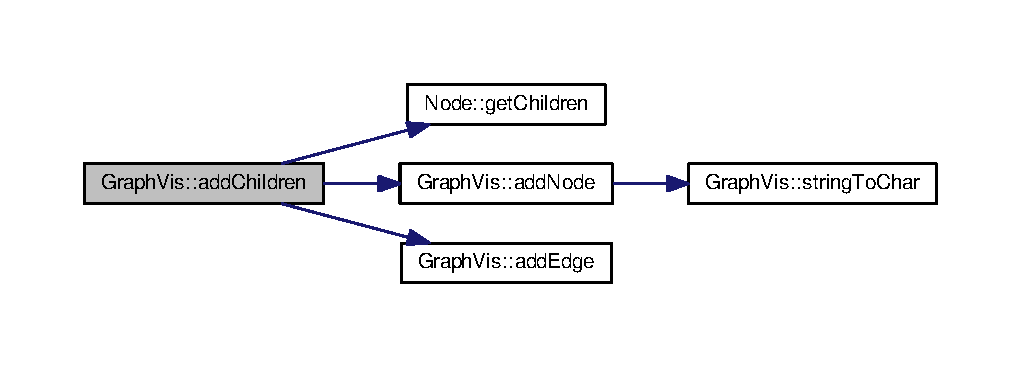
\includegraphics[width=350pt]{class_graph_vis_a683b40ddb0fdd31e0c39af23b9826aca_cgraph}
\end{center}
\end{figure}




Here is the caller graph for this function\-:
\nopagebreak
\begin{figure}[H]
\begin{center}
\leavevmode
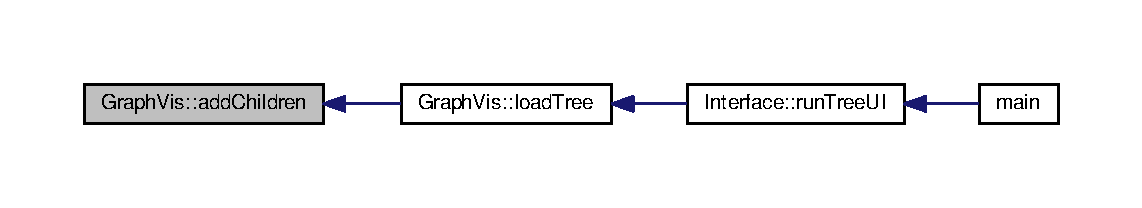
\includegraphics[width=350pt]{class_graph_vis_a683b40ddb0fdd31e0c39af23b9826aca_icgraph}
\end{center}
\end{figure}


\hypertarget{class_graph_vis_aa6403b7de690930c61d2c2ce50268bb1}{\index{Graph\-Vis@{Graph\-Vis}!add\-Edge@{add\-Edge}}
\index{add\-Edge@{add\-Edge}!GraphVis@{Graph\-Vis}}
\subsubsection[{add\-Edge}]{\setlength{\rightskip}{0pt plus 5cm}void Graph\-Vis\-::add\-Edge (
\begin{DoxyParamCaption}
\item[{Agnode\-\_\-t $\ast$}]{n1, }
\item[{Agnode\-\_\-t $\ast$}]{n2}
\end{DoxyParamCaption}
)}}\label{class_graph_vis_aa6403b7de690930c61d2c2ce50268bb1}


Adds an edge. 


\begin{DoxyParams}{Parameters}
{\em 2} & Agnode\-\_\-t$\ast$ that will be connected with an edge \\
\hline
\end{DoxyParams}


Definition at line 52 of file Graph\-Vis.\-cpp.



Here is the caller graph for this function\-:
\nopagebreak
\begin{figure}[H]
\begin{center}
\leavevmode
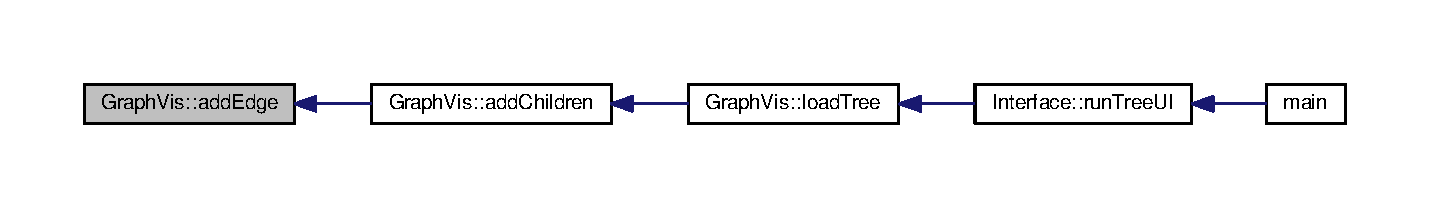
\includegraphics[width=350pt]{class_graph_vis_aa6403b7de690930c61d2c2ce50268bb1_icgraph}
\end{center}
\end{figure}


\hypertarget{class_graph_vis_aaadf4feb214a03fa6f923a30b7fcbf7f}{\index{Graph\-Vis@{Graph\-Vis}!add\-Node@{add\-Node}}
\index{add\-Node@{add\-Node}!GraphVis@{Graph\-Vis}}
\subsubsection[{add\-Node}]{\setlength{\rightskip}{0pt plus 5cm}Agnode\-\_\-t $\ast$ Graph\-Vis\-::add\-Node (
\begin{DoxyParamCaption}
\item[{std\-::string}]{name}
\end{DoxyParamCaption}
)}}\label{class_graph_vis_aaadf4feb214a03fa6f923a30b7fcbf7f}


Adds a node. 


\begin{DoxyParams}{Parameters}
{\em String} & containing the node's name \\
\hline
\end{DoxyParams}
\begin{DoxyReturn}{Returns}
Agnode\-\_\-t$\ast$ ready for use by graphviz 
\end{DoxyReturn}


Definition at line 34 of file Graph\-Vis.\-cpp.



Here is the call graph for this function\-:
\nopagebreak
\begin{figure}[H]
\begin{center}
\leavevmode
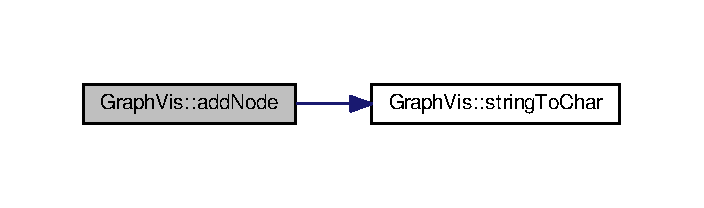
\includegraphics[width=338pt]{class_graph_vis_aaadf4feb214a03fa6f923a30b7fcbf7f_cgraph}
\end{center}
\end{figure}




Here is the caller graph for this function\-:
\nopagebreak
\begin{figure}[H]
\begin{center}
\leavevmode
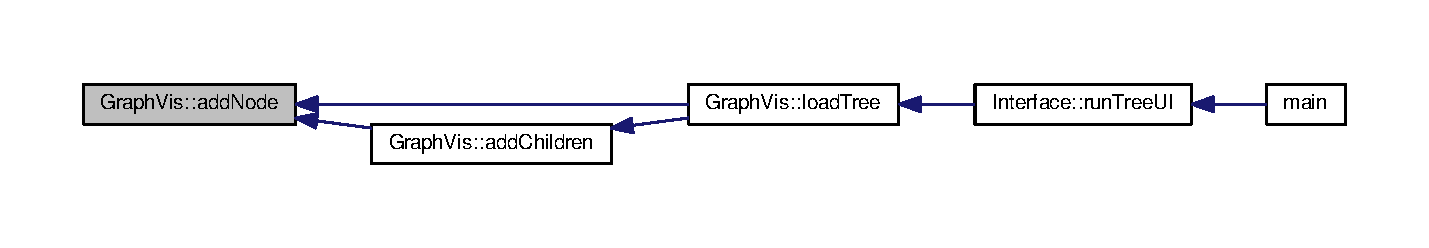
\includegraphics[width=350pt]{class_graph_vis_aaadf4feb214a03fa6f923a30b7fcbf7f_icgraph}
\end{center}
\end{figure}


\hypertarget{class_graph_vis_acab8c60a8f8b1a8fecd7297d303a2601}{\index{Graph\-Vis@{Graph\-Vis}!load\-Tree@{load\-Tree}}
\index{load\-Tree@{load\-Tree}!GraphVis@{Graph\-Vis}}
\subsubsection[{load\-Tree}]{\setlength{\rightskip}{0pt plus 5cm}void Graph\-Vis\-::load\-Tree (
\begin{DoxyParamCaption}
\item[{{\bf Tree} $\ast$}]{tree}
\end{DoxyParamCaption}
)}}\label{class_graph_vis_acab8c60a8f8b1a8fecd7297d303a2601}


Used to load a tree's nodes and call the appropriate function to output the png. 


\begin{DoxyParams}{Parameters}
{\em A} & pointer to a \hyperlink{class_tree}{Tree} class instance \\
\hline
\end{DoxyParams}


Definition at line 80 of file Graph\-Vis.\-cpp.



Here is the call graph for this function\-:
\nopagebreak
\begin{figure}[H]
\begin{center}
\leavevmode
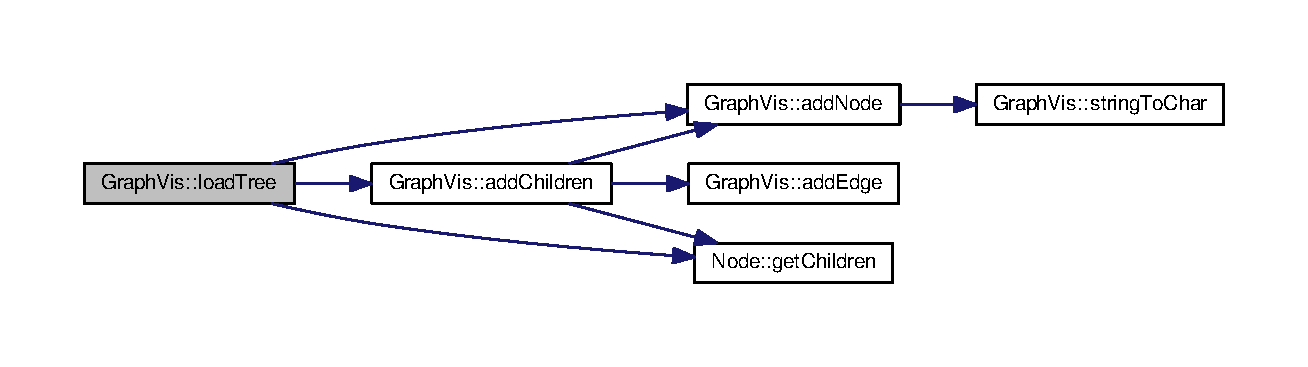
\includegraphics[width=350pt]{class_graph_vis_acab8c60a8f8b1a8fecd7297d303a2601_cgraph}
\end{center}
\end{figure}




Here is the caller graph for this function\-:
\nopagebreak
\begin{figure}[H]
\begin{center}
\leavevmode
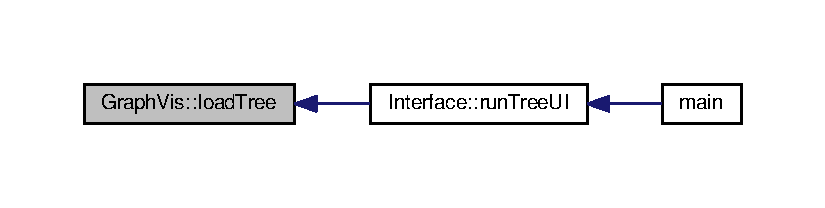
\includegraphics[width=350pt]{class_graph_vis_acab8c60a8f8b1a8fecd7297d303a2601_icgraph}
\end{center}
\end{figure}


\hypertarget{class_graph_vis_adcaebafcfc7696abfa49e894211e7077}{\index{Graph\-Vis@{Graph\-Vis}!string\-To\-Char@{string\-To\-Char}}
\index{string\-To\-Char@{string\-To\-Char}!GraphVis@{Graph\-Vis}}
\subsubsection[{string\-To\-Char}]{\setlength{\rightskip}{0pt plus 5cm}char $\ast$ Graph\-Vis\-::string\-To\-Char (
\begin{DoxyParamCaption}
\item[{std\-::string}]{input}
\end{DoxyParamCaption}
)\hspace{0.3cm}{\ttfamily [static]}}}\label{class_graph_vis_adcaebafcfc7696abfa49e894211e7077}


Converts a string variable to a char$\ast$ for graphviz compatibility reasons. 


\begin{DoxyParams}{Parameters}
{\em A} & string variable \\
\hline
\end{DoxyParams}


Definition at line 135 of file Graph\-Vis.\-cpp.



Here is the caller graph for this function\-:
\nopagebreak
\begin{figure}[H]
\begin{center}
\leavevmode
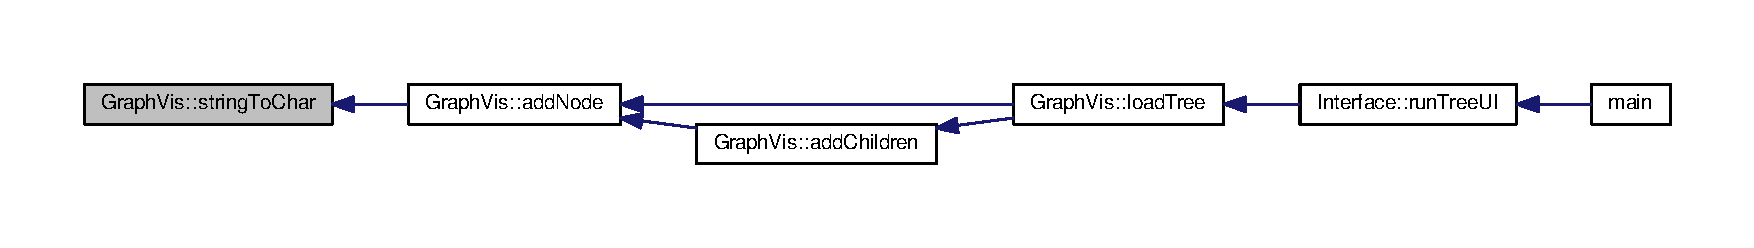
\includegraphics[width=350pt]{class_graph_vis_adcaebafcfc7696abfa49e894211e7077_icgraph}
\end{center}
\end{figure}


\hypertarget{class_graph_vis_a5606406187d65d9fb827ffe6df14b84e}{\index{Graph\-Vis@{Graph\-Vis}!write\-Graph\-To\-P\-N\-G@{write\-Graph\-To\-P\-N\-G}}
\index{write\-Graph\-To\-P\-N\-G@{write\-Graph\-To\-P\-N\-G}!GraphVis@{Graph\-Vis}}
\subsubsection[{write\-Graph\-To\-P\-N\-G}]{\setlength{\rightskip}{0pt plus 5cm}void Graph\-Vis\-::write\-Graph\-To\-P\-N\-G (
\begin{DoxyParamCaption}
\item[{std\-::string}]{filename}
\end{DoxyParamCaption}
)}}\label{class_graph_vis_a5606406187d65d9fb827ffe6df14b84e}


Transfers the tree to a png image. 


\begin{DoxyParams}{Parameters}
{\em Output} & image filename \\
\hline
\end{DoxyParams}


Definition at line 62 of file Graph\-Vis.\-cpp.



Here is the caller graph for this function\-:
\nopagebreak
\begin{figure}[H]
\begin{center}
\leavevmode
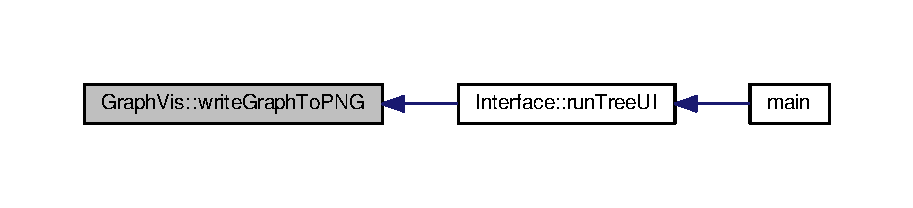
\includegraphics[width=350pt]{class_graph_vis_a5606406187d65d9fb827ffe6df14b84e_icgraph}
\end{center}
\end{figure}




The documentation for this class was generated from the following files\-:\begin{DoxyCompactItemize}
\item 
/home/baios/\-Coding/\-C++/\-Git\-Data\-Structures/\-Data\-Structures/234\-Tree/include/\hyperlink{_graph_vis_8h}{Graph\-Vis.\-h}\item 
/home/baios/\-Coding/\-C++/\-Git\-Data\-Structures/\-Data\-Structures/234\-Tree/src/\hyperlink{_graph_vis_8cpp}{Graph\-Vis.\-cpp}\end{DoxyCompactItemize}

\hypertarget{class_interface}{\section{Interface Class Reference}
\label{class_interface}\index{Interface@{Interface}}
}


\hyperlink{class_interface}{Interface} Class.  




{\ttfamily \#include $<$Interface.\-h$>$}

\subsection*{Public Member Functions}
\begin{DoxyCompactItemize}
\item 
\hyperlink{class_interface_a4406d74c75bdfe150bf72be1f1cda8b1}{Interface} ()
\begin{DoxyCompactList}\small\item\em Instanciates a \hyperlink{class_tree}{Tree} object for use later on. \end{DoxyCompactList}\item 
void \hyperlink{class_interface_a39dfccfcfc9027f148f1a0280ff34fe5}{run\-Tree\-U\-I} ()
\begin{DoxyCompactList}\small\item\em Prints a basic menu to the user with all the available function that can be invoked on the tree. \end{DoxyCompactList}\item 
\hyperlink{class_tree}{Tree} $\ast$ \hyperlink{class_interface_a52fce95d6f5f1060df253df752ef89e2}{get\-Tree} ()
\end{DoxyCompactItemize}


\subsection{Detailed Description}
\hyperlink{class_interface}{Interface} Class. 

This class is basicaly a C\-L\-I implementation so that the user can easily manage the tree and/or add/remove nodes. The user can also request values concerning the tree's current state. The class offers a sample tree option for quick testing

\begin{DoxyAuthor}{Author}
Vaios Papaspyros
\end{DoxyAuthor}
Contact\-: \href{mailto:b.papaspyros@gmail.com}{\tt b.\-papaspyros@gmail.\-com} or create an issue on the github page \href{https://github.com/bpapaspyros/DataStructures}{\tt https\-://github.\-com/bpapaspyros/\-Data\-Structures} 

Definition at line 21 of file Interface.\-h.



\subsection{Constructor \& Destructor Documentation}
\hypertarget{class_interface_a4406d74c75bdfe150bf72be1f1cda8b1}{\index{Interface@{Interface}!Interface@{Interface}}
\index{Interface@{Interface}!Interface@{Interface}}
\subsubsection[{Interface}]{\setlength{\rightskip}{0pt plus 5cm}Interface\-::\-Interface (
\begin{DoxyParamCaption}
{}
\end{DoxyParamCaption}
)}}\label{class_interface_a4406d74c75bdfe150bf72be1f1cda8b1}


Instanciates a \hyperlink{class_tree}{Tree} object for use later on. 



Definition at line 9 of file Interface.\-cpp.



\subsection{Member Function Documentation}
\hypertarget{class_interface_a52fce95d6f5f1060df253df752ef89e2}{\index{Interface@{Interface}!get\-Tree@{get\-Tree}}
\index{get\-Tree@{get\-Tree}!Interface@{Interface}}
\subsubsection[{get\-Tree}]{\setlength{\rightskip}{0pt plus 5cm}{\bf Tree} $\ast$ Interface\-::get\-Tree (
\begin{DoxyParamCaption}
{}
\end{DoxyParamCaption}
)}}\label{class_interface_a52fce95d6f5f1060df253df752ef89e2}
\begin{DoxyReturn}{Returns}
Returns a pointer to the whole tree 
\end{DoxyReturn}


Definition at line 202 of file Interface.\-cpp.

\hypertarget{class_interface_a39dfccfcfc9027f148f1a0280ff34fe5}{\index{Interface@{Interface}!run\-Tree\-U\-I@{run\-Tree\-U\-I}}
\index{run\-Tree\-U\-I@{run\-Tree\-U\-I}!Interface@{Interface}}
\subsubsection[{run\-Tree\-U\-I}]{\setlength{\rightskip}{0pt plus 5cm}void Interface\-::run\-Tree\-U\-I (
\begin{DoxyParamCaption}
{}
\end{DoxyParamCaption}
)}}\label{class_interface_a39dfccfcfc9027f148f1a0280ff34fe5}


Prints a basic menu to the user with all the available function that can be invoked on the tree. 



Definition at line 14 of file Interface.\-cpp.



Here is the call graph for this function\-:
\nopagebreak
\begin{figure}[H]
\begin{center}
\leavevmode
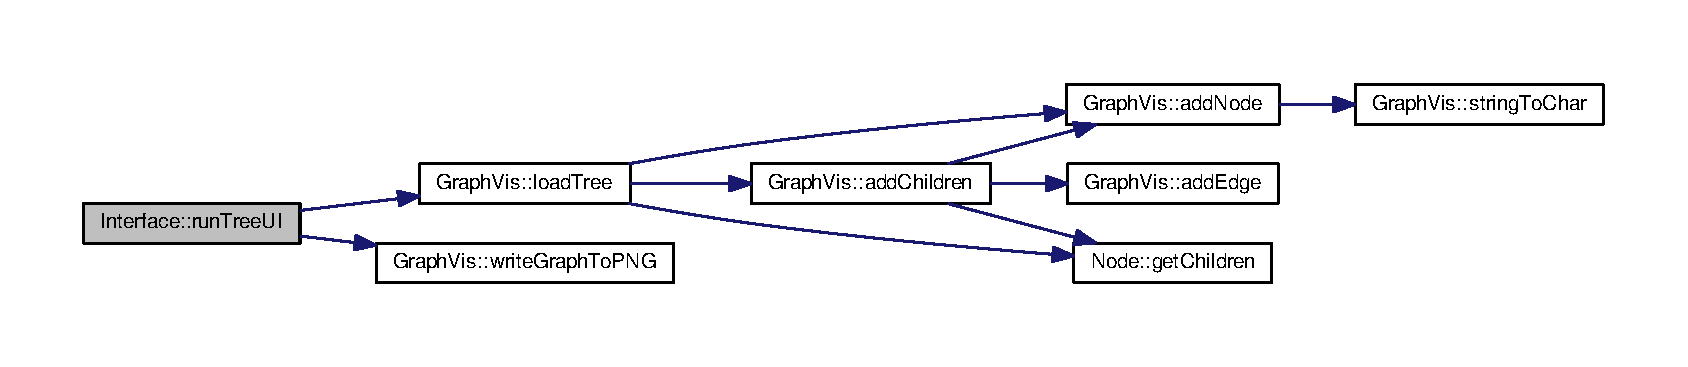
\includegraphics[width=350pt]{class_interface_a39dfccfcfc9027f148f1a0280ff34fe5_cgraph}
\end{center}
\end{figure}




Here is the caller graph for this function\-:\nopagebreak
\begin{figure}[H]
\begin{center}
\leavevmode
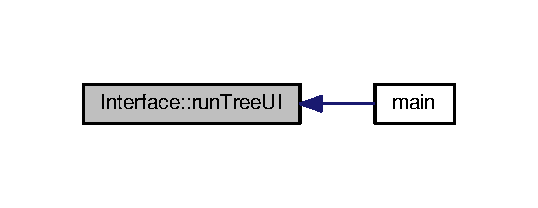
\includegraphics[width=258pt]{class_interface_a39dfccfcfc9027f148f1a0280ff34fe5_icgraph}
\end{center}
\end{figure}




The documentation for this class was generated from the following files\-:\begin{DoxyCompactItemize}
\item 
/home/baios/\-Coding/\-C++/\-Git\-Data\-Structures/\-Data\-Structures/234\-Tree/include/\hyperlink{_interface_8h}{Interface.\-h}\item 
/home/baios/\-Coding/\-C++/\-Git\-Data\-Structures/\-Data\-Structures/234\-Tree/src/\hyperlink{_interface_8cpp}{Interface.\-cpp}\end{DoxyCompactItemize}

\hypertarget{class_node}{\section{Node Class Reference}
\label{class_node}\index{Node@{Node}}
}


\hyperlink{class_node}{Node} Class.  




{\ttfamily \#include $<$Node.\-h$>$}



Collaboration diagram for Node\-:\nopagebreak
\begin{figure}[H]
\begin{center}
\leavevmode
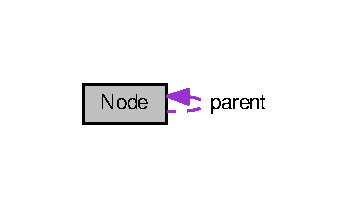
\includegraphics[width=169pt]{class_node__coll__graph}
\end{center}
\end{figure}
\subsection*{Public Member Functions}
\begin{DoxyCompactItemize}
\item 
\hyperlink{class_node_a9524dc2afb2e7343951a4244edfd7621}{Node} (int data, \hyperlink{class_node}{Node} $\ast$p)
\begin{DoxyCompactList}\small\item\em The constructor adds the data given as parameter to the data vector and sets the current node's parent. \end{DoxyCompactList}\item 
\hyperlink{class_node_aa0840c3cb5c7159be6d992adecd2097c}{$\sim$\-Node} ()
\begin{DoxyCompactList}\small\item\em The destructor deletes all members of the children vector when the instance goes out of scope. \end{DoxyCompactList}\item 
int \hyperlink{class_node_ac393c36db7ebed00ac390e97f9994a12}{get\-Children} ()
\begin{DoxyCompactList}\small\item\em Returns the number of children for this node instance. \end{DoxyCompactList}\item 
bool \hyperlink{class_node_a3a61dca67d5ad06cacb8c48eb6374973}{is\-Leaf} ()
\begin{DoxyCompactList}\small\item\em Depending on whether the current node is a leaf or not it returns a boolean value. \end{DoxyCompactList}\item 
void \hyperlink{class_node_a934927d1194b331bf502daea96513eef}{insert\-Child} (\hyperlink{class_node}{Node} $\ast$child)
\begin{DoxyCompactList}\small\item\em Pushes a node to the children vector. \end{DoxyCompactList}\item 
int \hyperlink{class_node_a7c98fb9df43ac39b5e74eda16434908b}{recursive\-Num\-Of\-Nodes} (\hyperlink{class_node}{Node} $\ast$n)
\begin{DoxyCompactList}\small\item\em Counts the number of nodes recursively. \end{DoxyCompactList}\item 
int \hyperlink{class_node_a970755e7b9ff4a33fde5433663f06549}{recursive\-Num\-Of\-Leaves} (\hyperlink{class_node}{Node} $\ast$n)
\begin{DoxyCompactList}\small\item\em Counts the number of leaves recursively. \end{DoxyCompactList}\item 
int $\ast$ \hyperlink{class_node_ae0c0332615644c989be5c8137b4109a5}{recursive\-Int\-Array} (\hyperlink{class_node}{Node} $\ast$n)
\begin{DoxyCompactList}\small\item\em Creates an array of integers with the info located in the leaves. The array should be sorted if the tree is balanced correctly. \end{DoxyCompactList}\end{DoxyCompactItemize}
\subsection*{Public Attributes}
\begin{DoxyCompactItemize}
\item 
std\-::vector$<$ \hyperlink{class_node}{Node} $\ast$ $>$ \hyperlink{class_node_a49baf1d613dc14f1e1e4aad883dde6fe}{children}
\begin{DoxyCompactList}\small\item\em Pointers to children. \end{DoxyCompactList}\item 
std\-::vector$<$ int $>$ \hyperlink{class_node_aebcdeef2d940bb25316fd0eac5d51ed2}{\-\_\-data}
\begin{DoxyCompactList}\small\item\em \hyperlink{class_node}{Node} data. \end{DoxyCompactList}\item 
\hyperlink{class_node}{Node} $\ast$ \hyperlink{class_node_ad8184598cdea70e4bbdfd76f2b0f9e85}{parent}
\begin{DoxyCompactList}\small\item\em Pointer to parent. \end{DoxyCompactList}\end{DoxyCompactItemize}


\subsection{Detailed Description}
\hyperlink{class_node}{Node} Class. 

This class has methods tha let you manage the node (children, data) and give you significant functions to calculate tree values and others that let you iterate through the tree

\begin{DoxyAuthor}{Author}
Vaios Papaspyros
\end{DoxyAuthor}
Contact\-: \href{mailto:b.papaspyros@gmail.com}{\tt b.\-papaspyros@gmail.\-com} or create an issue on the github page \href{https://github.com/bpapaspyros/DataStructures}{\tt https\-://github.\-com/bpapaspyros/\-Data\-Structures} 

Definition at line 21 of file Node.\-h.



\subsection{Constructor \& Destructor Documentation}
\hypertarget{class_node_a9524dc2afb2e7343951a4244edfd7621}{\index{Node@{Node}!Node@{Node}}
\index{Node@{Node}!Node@{Node}}
\subsubsection[{Node}]{\setlength{\rightskip}{0pt plus 5cm}Node\-::\-Node (
\begin{DoxyParamCaption}
\item[{int}]{data, }
\item[{{\bf Node} $\ast$}]{p}
\end{DoxyParamCaption}
)}}\label{class_node_a9524dc2afb2e7343951a4244edfd7621}


The constructor adds the data given as parameter to the data vector and sets the current node's parent. 


\begin{DoxyParams}{Parameters}
{\em Takes} & an integer data which stands for the node key and a pointer to a \hyperlink{class_node}{Node} class instance \\
\hline
\end{DoxyParams}


Definition at line 10 of file Node.\-cpp.

\hypertarget{class_node_aa0840c3cb5c7159be6d992adecd2097c}{\index{Node@{Node}!$\sim$\-Node@{$\sim$\-Node}}
\index{$\sim$\-Node@{$\sim$\-Node}!Node@{Node}}
\subsubsection[{$\sim$\-Node}]{\setlength{\rightskip}{0pt plus 5cm}Node\-::$\sim$\-Node (
\begin{DoxyParamCaption}
{}
\end{DoxyParamCaption}
)}}\label{class_node_aa0840c3cb5c7159be6d992adecd2097c}


The destructor deletes all members of the children vector when the instance goes out of scope. 



Definition at line 24 of file Node.\-cpp.



Here is the call graph for this function\-:
\nopagebreak
\begin{figure}[H]
\begin{center}
\leavevmode
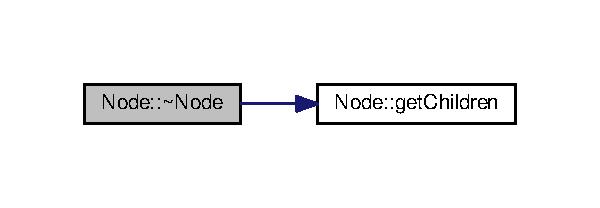
\includegraphics[width=288pt]{class_node_aa0840c3cb5c7159be6d992adecd2097c_cgraph}
\end{center}
\end{figure}




\subsection{Member Function Documentation}
\hypertarget{class_node_ac393c36db7ebed00ac390e97f9994a12}{\index{Node@{Node}!get\-Children@{get\-Children}}
\index{get\-Children@{get\-Children}!Node@{Node}}
\subsubsection[{get\-Children}]{\setlength{\rightskip}{0pt plus 5cm}int Node\-::get\-Children (
\begin{DoxyParamCaption}
{}
\end{DoxyParamCaption}
)}}\label{class_node_ac393c36db7ebed00ac390e97f9994a12}


Returns the number of children for this node instance. 

\begin{DoxyReturn}{Returns}
the number of children for this node instance 
\end{DoxyReturn}


Definition at line 113 of file Node.\-cpp.



Here is the caller graph for this function\-:
\nopagebreak
\begin{figure}[H]
\begin{center}
\leavevmode
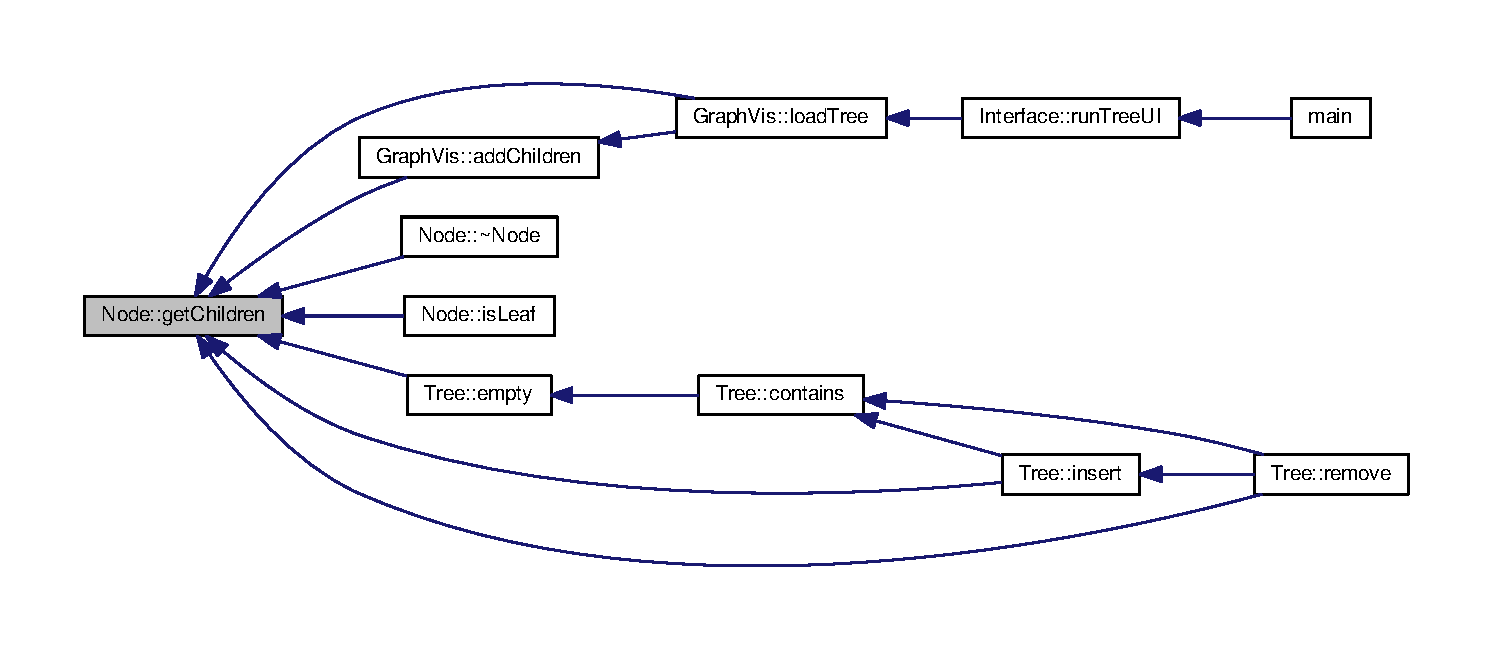
\includegraphics[width=350pt]{class_node_ac393c36db7ebed00ac390e97f9994a12_icgraph}
\end{center}
\end{figure}


\hypertarget{class_node_a934927d1194b331bf502daea96513eef}{\index{Node@{Node}!insert\-Child@{insert\-Child}}
\index{insert\-Child@{insert\-Child}!Node@{Node}}
\subsubsection[{insert\-Child}]{\setlength{\rightskip}{0pt plus 5cm}void Node\-::insert\-Child (
\begin{DoxyParamCaption}
\item[{{\bf Node} $\ast$}]{child}
\end{DoxyParamCaption}
)}}\label{class_node_a934927d1194b331bf502daea96513eef}


Pushes a node to the children vector. 


\begin{DoxyParams}{Parameters}
{\em Takes} & a pointer to a node instance \\
\hline
\end{DoxyParams}


Definition at line 136 of file Node.\-cpp.



Here is the caller graph for this function\-:
\nopagebreak
\begin{figure}[H]
\begin{center}
\leavevmode
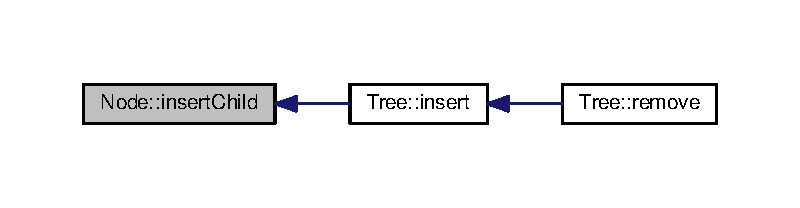
\includegraphics[width=350pt]{class_node_a934927d1194b331bf502daea96513eef_icgraph}
\end{center}
\end{figure}


\hypertarget{class_node_a3a61dca67d5ad06cacb8c48eb6374973}{\index{Node@{Node}!is\-Leaf@{is\-Leaf}}
\index{is\-Leaf@{is\-Leaf}!Node@{Node}}
\subsubsection[{is\-Leaf}]{\setlength{\rightskip}{0pt plus 5cm}bool Node\-::is\-Leaf (
\begin{DoxyParamCaption}
{}
\end{DoxyParamCaption}
)}}\label{class_node_a3a61dca67d5ad06cacb8c48eb6374973}


Depending on whether the current node is a leaf or not it returns a boolean value. 

\begin{DoxyReturn}{Returns}
Returns true if this node is in fact a leaf or false otherwise 
\end{DoxyReturn}


Definition at line 123 of file Node.\-cpp.



Here is the call graph for this function\-:
\nopagebreak
\begin{figure}[H]
\begin{center}
\leavevmode
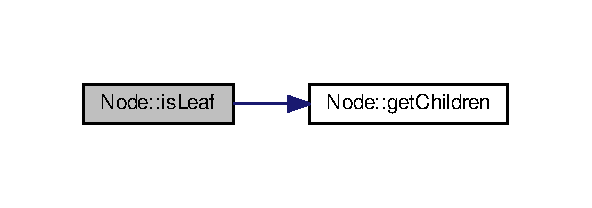
\includegraphics[width=284pt]{class_node_a3a61dca67d5ad06cacb8c48eb6374973_cgraph}
\end{center}
\end{figure}


\hypertarget{class_node_ae0c0332615644c989be5c8137b4109a5}{\index{Node@{Node}!recursive\-Int\-Array@{recursive\-Int\-Array}}
\index{recursive\-Int\-Array@{recursive\-Int\-Array}!Node@{Node}}
\subsubsection[{recursive\-Int\-Array}]{\setlength{\rightskip}{0pt plus 5cm}int $\ast$ Node\-::recursive\-Int\-Array (
\begin{DoxyParamCaption}
\item[{{\bf Node} $\ast$}]{n}
\end{DoxyParamCaption}
)}}\label{class_node_ae0c0332615644c989be5c8137b4109a5}


Creates an array of integers with the info located in the leaves. The array should be sorted if the tree is balanced correctly. 


\begin{DoxyParams}{Parameters}
{\em Takes} & a pointer to a node instance \\
\hline
\end{DoxyParams}
\begin{DoxyReturn}{Returns}
Returns an array of integers with the leaf content 
\end{DoxyReturn}


Definition at line 83 of file Node.\-cpp.



Here is the call graph for this function\-:
\nopagebreak
\begin{figure}[H]
\begin{center}
\leavevmode
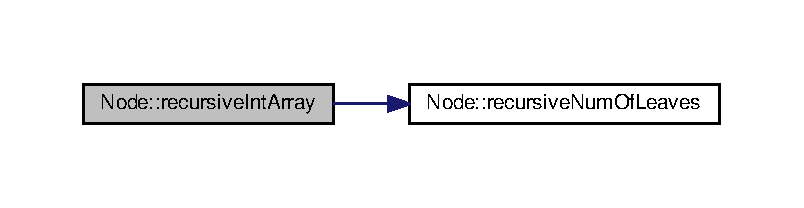
\includegraphics[width=350pt]{class_node_ae0c0332615644c989be5c8137b4109a5_cgraph}
\end{center}
\end{figure}




Here is the caller graph for this function\-:
\nopagebreak
\begin{figure}[H]
\begin{center}
\leavevmode
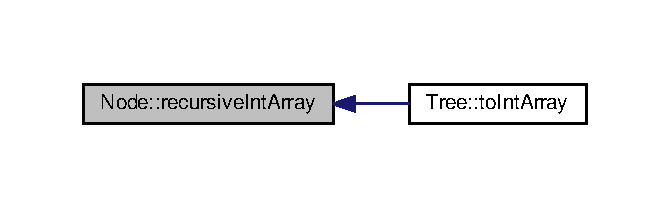
\includegraphics[width=322pt]{class_node_ae0c0332615644c989be5c8137b4109a5_icgraph}
\end{center}
\end{figure}


\hypertarget{class_node_a970755e7b9ff4a33fde5433663f06549}{\index{Node@{Node}!recursive\-Num\-Of\-Leaves@{recursive\-Num\-Of\-Leaves}}
\index{recursive\-Num\-Of\-Leaves@{recursive\-Num\-Of\-Leaves}!Node@{Node}}
\subsubsection[{recursive\-Num\-Of\-Leaves}]{\setlength{\rightskip}{0pt plus 5cm}int Node\-::recursive\-Num\-Of\-Leaves (
\begin{DoxyParamCaption}
\item[{{\bf Node} $\ast$}]{n}
\end{DoxyParamCaption}
)}}\label{class_node_a970755e7b9ff4a33fde5433663f06549}


Counts the number of leaves recursively. 


\begin{DoxyParams}{Parameters}
{\em Takes} & a pointer to a node instance \\
\hline
\end{DoxyParams}
\begin{DoxyReturn}{Returns}
Returns the number of leaves in the tree (int) 
\end{DoxyReturn}


Definition at line 61 of file Node.\-cpp.



Here is the caller graph for this function\-:
\nopagebreak
\begin{figure}[H]
\begin{center}
\leavevmode
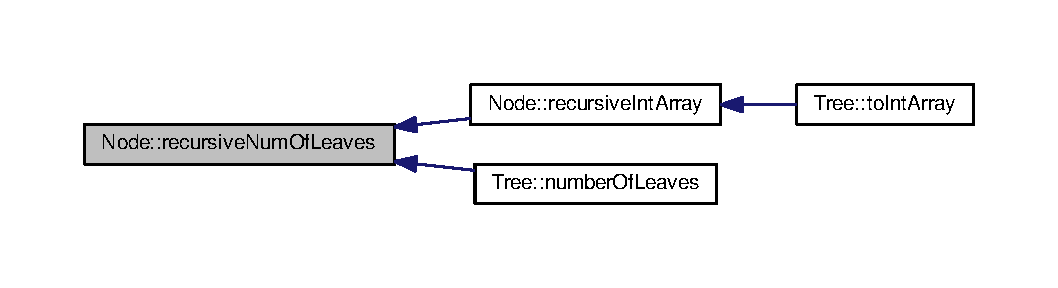
\includegraphics[width=350pt]{class_node_a970755e7b9ff4a33fde5433663f06549_icgraph}
\end{center}
\end{figure}


\hypertarget{class_node_a7c98fb9df43ac39b5e74eda16434908b}{\index{Node@{Node}!recursive\-Num\-Of\-Nodes@{recursive\-Num\-Of\-Nodes}}
\index{recursive\-Num\-Of\-Nodes@{recursive\-Num\-Of\-Nodes}!Node@{Node}}
\subsubsection[{recursive\-Num\-Of\-Nodes}]{\setlength{\rightskip}{0pt plus 5cm}int Node\-::recursive\-Num\-Of\-Nodes (
\begin{DoxyParamCaption}
\item[{{\bf Node} $\ast$}]{n}
\end{DoxyParamCaption}
)}}\label{class_node_a7c98fb9df43ac39b5e74eda16434908b}


Counts the number of nodes recursively. 


\begin{DoxyParams}{Parameters}
{\em Takes} & a pointer to a node instance \\
\hline
\end{DoxyParams}
\begin{DoxyReturn}{Returns}
Returns the number of nodes in the tree (int) 
\end{DoxyReturn}


Definition at line 35 of file Node.\-cpp.



Here is the caller graph for this function\-:
\nopagebreak
\begin{figure}[H]
\begin{center}
\leavevmode
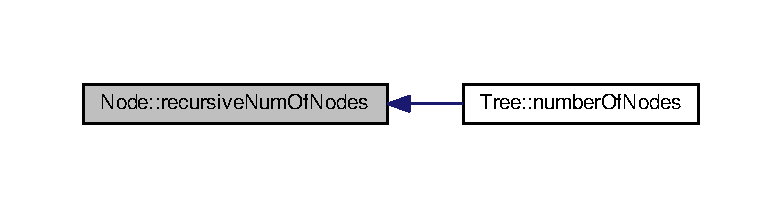
\includegraphics[width=350pt]{class_node_a7c98fb9df43ac39b5e74eda16434908b_icgraph}
\end{center}
\end{figure}




\subsection{Member Data Documentation}
\hypertarget{class_node_aebcdeef2d940bb25316fd0eac5d51ed2}{\index{Node@{Node}!\-\_\-data@{\-\_\-data}}
\index{\-\_\-data@{\-\_\-data}!Node@{Node}}
\subsubsection[{\-\_\-data}]{\setlength{\rightskip}{0pt plus 5cm}std\-::vector$<$int$>$ Node\-::\-\_\-data}}\label{class_node_aebcdeef2d940bb25316fd0eac5d51ed2}


\hyperlink{class_node}{Node} data. 



Definition at line 72 of file Node.\-h.

\hypertarget{class_node_a49baf1d613dc14f1e1e4aad883dde6fe}{\index{Node@{Node}!children@{children}}
\index{children@{children}!Node@{Node}}
\subsubsection[{children}]{\setlength{\rightskip}{0pt plus 5cm}std\-::vector$<${\bf Node}$\ast$$>$ Node\-::children}}\label{class_node_a49baf1d613dc14f1e1e4aad883dde6fe}


Pointers to children. 



Definition at line 69 of file Node.\-h.

\hypertarget{class_node_ad8184598cdea70e4bbdfd76f2b0f9e85}{\index{Node@{Node}!parent@{parent}}
\index{parent@{parent}!Node@{Node}}
\subsubsection[{parent}]{\setlength{\rightskip}{0pt plus 5cm}{\bf Node}$\ast$ Node\-::parent}}\label{class_node_ad8184598cdea70e4bbdfd76f2b0f9e85}


Pointer to parent. 



Definition at line 75 of file Node.\-h.



The documentation for this class was generated from the following files\-:\begin{DoxyCompactItemize}
\item 
/home/baios/\-Coding/\-C++/\-Git\-Data\-Structures/\-Data\-Structures/234\-Tree/include/\hyperlink{_node_8h}{Node.\-h}\item 
/home/baios/\-Coding/\-C++/\-Git\-Data\-Structures/\-Data\-Structures/234\-Tree/src/\hyperlink{_node_8cpp}{Node.\-cpp}\end{DoxyCompactItemize}

\hypertarget{class_tree}{\section{Tree Class Reference}
\label{class_tree}\index{Tree@{Tree}}
}


\hyperlink{class_tree}{Tree} Class.  




{\ttfamily \#include $<$Tree.\-h$>$}



Collaboration diagram for Tree\-:
\nopagebreak
\begin{figure}[H]
\begin{center}
\leavevmode
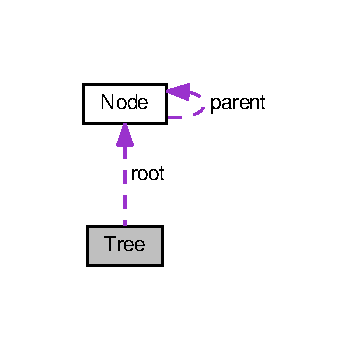
\includegraphics[width=169pt]{class_tree__coll__graph}
\end{center}
\end{figure}
\subsection*{Public Member Functions}
\begin{DoxyCompactItemize}
\item 
\hyperlink{class_tree_ad376a7c639d857312f5de2ef47482f68}{Tree} ()
\item 
\hyperlink{class_tree_ad913989ea4c1195b32b2082860560bf0}{Tree} (\hyperlink{class_node}{Node} $\ast$node)
\begin{DoxyCompactList}\small\item\em Initializes the tree with another tree. \end{DoxyCompactList}\item 
\hyperlink{class_tree_abdc38545cf3f588725b5d8b8075b3866}{$\sim$\-Tree} ()
\item 
bool \hyperlink{class_tree_a853993d1cc8acbf1ca26a98bc50e3795}{empty} ()
\item 
bool \hyperlink{class_tree_abb768469ad246c52c8b5ba6ad9c02f70}{contains} (int key)
\begin{DoxyCompactList}\small\item\em Simply checks if the given value is contained in the tree as a leaf. \end{DoxyCompactList}\item 
void \hyperlink{class_tree_a0b32b0ca65d8ef7df1dc3a1bd0cf6a99}{insert} (int key)
\begin{DoxyCompactList}\small\item\em Inserts the requested value to the tree as a leaf while keeping it balanced. \end{DoxyCompactList}\item 
void \hyperlink{class_tree_a0015486626ad4da2a7dba4f60ed9aa79}{remove} (int key)
\begin{DoxyCompactList}\small\item\em Removes the requested leaf while keeping the tree balanced. \end{DoxyCompactList}\item 
int \hyperlink{class_tree_a455b10d21349072737b951ad34c2311a}{number\-Of\-Nodes} ()
\begin{DoxyCompactList}\small\item\em Counting the number of nodes that the tree holds with a recursive function. \end{DoxyCompactList}\item 
int $\ast$ \hyperlink{class_tree_a730a56b16e855a1b08a24ee11840d508}{to\-Int\-Array} ()
\begin{DoxyCompactList}\small\item\em An array containing all the info from the leaves. \end{DoxyCompactList}\item 
int \hyperlink{class_tree_a54ddf4e99c00553a6b07cb9b149988e2}{number\-Of\-Leaves} ()
\begin{DoxyCompactList}\small\item\em Counting the number of leaves that the tree holds with a recursive function. \end{DoxyCompactList}\item 
void \hyperlink{class_tree_a8a64e556c6fc5da582739c3c80d65600}{leaf\-Info\-To\-File} (int $\ast$in\-Array, int size)
\begin{DoxyCompactList}\small\item\em Writes the leaf info to text file. \end{DoxyCompactList}\item 
void \hyperlink{class_tree_ad1a1d70cd502cbdc0635a0921199fcfb}{init\-Root\-Keys} ()
\begin{DoxyCompactList}\small\item\em Initializes the root keys. \end{DoxyCompactList}\end{DoxyCompactItemize}
\subsection*{Public Attributes}
\begin{DoxyCompactItemize}
\item 
\hyperlink{class_node}{Node} $\ast$ \hyperlink{class_tree_ad8e46ce0aead5778cbdd784d1e370d5f}{root}
\end{DoxyCompactItemize}


\subsection{Detailed Description}
\hyperlink{class_tree}{Tree} Class. 

This class contains methods that execute the fundamental tree functions such as add, remove, etc. There are also methods that calculate tree related values, such as the number of nodes or leaves. An additional method offers functionality for writing the tree data to a file.

\begin{DoxyAuthor}{Author}
Vaios Papaspyros
\end{DoxyAuthor}
Contact\-: \href{mailto:b.papaspyros@gmail.com}{\tt b.\-papaspyros@gmail.\-com} or create an issue on the github page \href{https://github.com/bpapaspyros/DataStructures}{\tt https\-://github.\-com/bpapaspyros/\-Data\-Structures} 

Definition at line 24 of file Tree.\-h.



\subsection{Constructor \& Destructor Documentation}
\hypertarget{class_tree_ad376a7c639d857312f5de2ef47482f68}{\index{Tree@{Tree}!Tree@{Tree}}
\index{Tree@{Tree}!Tree@{Tree}}
\subsubsection[{Tree}]{\setlength{\rightskip}{0pt plus 5cm}Tree\-::\-Tree (
\begin{DoxyParamCaption}
{}
\end{DoxyParamCaption}
)}}\label{class_tree_ad376a7c639d857312f5de2ef47482f68}


Definition at line 5 of file Tree.\-cpp.

\hypertarget{class_tree_ad913989ea4c1195b32b2082860560bf0}{\index{Tree@{Tree}!Tree@{Tree}}
\index{Tree@{Tree}!Tree@{Tree}}
\subsubsection[{Tree}]{\setlength{\rightskip}{0pt plus 5cm}Tree\-::\-Tree (
\begin{DoxyParamCaption}
\item[{{\bf Node} $\ast$}]{node}
\end{DoxyParamCaption}
)}}\label{class_tree_ad913989ea4c1195b32b2082860560bf0}


Initializes the tree with another tree. 


\begin{DoxyParams}{Parameters}
{\em Takes} & a Node$\ast$ \\
\hline
\end{DoxyParams}


Definition at line 11 of file Tree.\-cpp.

\hypertarget{class_tree_abdc38545cf3f588725b5d8b8075b3866}{\index{Tree@{Tree}!$\sim$\-Tree@{$\sim$\-Tree}}
\index{$\sim$\-Tree@{$\sim$\-Tree}!Tree@{Tree}}
\subsubsection[{$\sim$\-Tree}]{\setlength{\rightskip}{0pt plus 5cm}Tree\-::$\sim$\-Tree (
\begin{DoxyParamCaption}
{}
\end{DoxyParamCaption}
)}}\label{class_tree_abdc38545cf3f588725b5d8b8075b3866}


Definition at line 17 of file Tree.\-cpp.



\subsection{Member Function Documentation}
\hypertarget{class_tree_abb768469ad246c52c8b5ba6ad9c02f70}{\index{Tree@{Tree}!contains@{contains}}
\index{contains@{contains}!Tree@{Tree}}
\subsubsection[{contains}]{\setlength{\rightskip}{0pt plus 5cm}bool Tree\-::contains (
\begin{DoxyParamCaption}
\item[{int}]{key}
\end{DoxyParamCaption}
)}}\label{class_tree_abb768469ad246c52c8b5ba6ad9c02f70}


Simply checks if the given value is contained in the tree as a leaf. 


\begin{DoxyParams}{Parameters}
{\em Takes} & an integer that stands for the element we are looking for \\
\hline
\end{DoxyParams}
\begin{DoxyReturn}{Returns}
Returns tree if the given value exists in the tree 
\end{DoxyReturn}


Definition at line 33 of file Tree.\-cpp.



Here is the call graph for this function\-:
\nopagebreak
\begin{figure}[H]
\begin{center}
\leavevmode
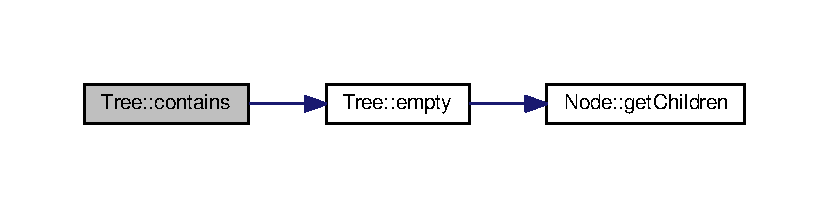
\includegraphics[width=350pt]{class_tree_abb768469ad246c52c8b5ba6ad9c02f70_cgraph}
\end{center}
\end{figure}




Here is the caller graph for this function\-:
\nopagebreak
\begin{figure}[H]
\begin{center}
\leavevmode
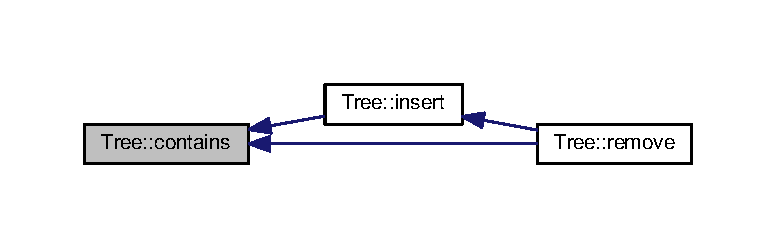
\includegraphics[width=350pt]{class_tree_abb768469ad246c52c8b5ba6ad9c02f70_icgraph}
\end{center}
\end{figure}


\hypertarget{class_tree_a853993d1cc8acbf1ca26a98bc50e3795}{\index{Tree@{Tree}!empty@{empty}}
\index{empty@{empty}!Tree@{Tree}}
\subsubsection[{empty}]{\setlength{\rightskip}{0pt plus 5cm}bool Tree\-::empty (
\begin{DoxyParamCaption}
{}
\end{DoxyParamCaption}
)}}\label{class_tree_a853993d1cc8acbf1ca26a98bc50e3795}
brief Just checking if the tree is empty or not \begin{DoxyReturn}{Returns}
Returns true if the tree is empty of nodes, otherwiese returns false 
\end{DoxyReturn}


Definition at line 23 of file Tree.\-cpp.



Here is the call graph for this function\-:
\nopagebreak
\begin{figure}[H]
\begin{center}
\leavevmode
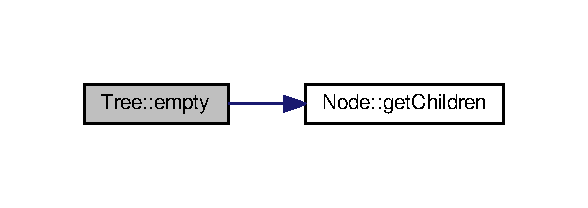
\includegraphics[width=282pt]{class_tree_a853993d1cc8acbf1ca26a98bc50e3795_cgraph}
\end{center}
\end{figure}




Here is the caller graph for this function\-:
\nopagebreak
\begin{figure}[H]
\begin{center}
\leavevmode
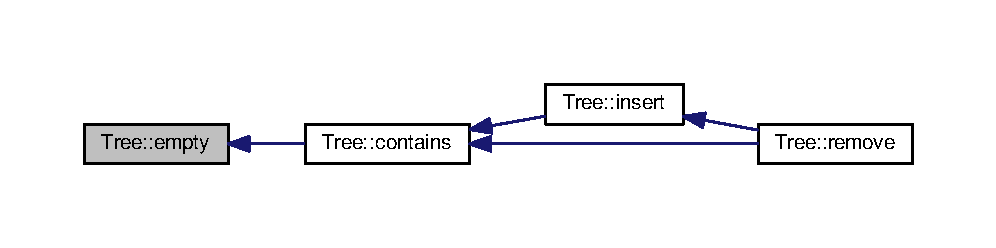
\includegraphics[width=350pt]{class_tree_a853993d1cc8acbf1ca26a98bc50e3795_icgraph}
\end{center}
\end{figure}


\hypertarget{class_tree_ad1a1d70cd502cbdc0635a0921199fcfb}{\index{Tree@{Tree}!init\-Root\-Keys@{init\-Root\-Keys}}
\index{init\-Root\-Keys@{init\-Root\-Keys}!Tree@{Tree}}
\subsubsection[{init\-Root\-Keys}]{\setlength{\rightskip}{0pt plus 5cm}void Tree\-::init\-Root\-Keys (
\begin{DoxyParamCaption}
{}
\end{DoxyParamCaption}
)}}\label{class_tree_ad1a1d70cd502cbdc0635a0921199fcfb}


Initializes the root keys. 



Definition at line 350 of file Tree.\-cpp.

\hypertarget{class_tree_a0b32b0ca65d8ef7df1dc3a1bd0cf6a99}{\index{Tree@{Tree}!insert@{insert}}
\index{insert@{insert}!Tree@{Tree}}
\subsubsection[{insert}]{\setlength{\rightskip}{0pt plus 5cm}void Tree\-::insert (
\begin{DoxyParamCaption}
\item[{int}]{key}
\end{DoxyParamCaption}
)}}\label{class_tree_a0b32b0ca65d8ef7df1dc3a1bd0cf6a99}


Inserts the requested value to the tree as a leaf while keeping it balanced. 


\begin{DoxyParams}{Parameters}
{\em Integer} & value to be added to the tree as a leaf \\
\hline
\end{DoxyParams}


Definition at line 59 of file Tree.\-cpp.



Here is the call graph for this function\-:
\nopagebreak
\begin{figure}[H]
\begin{center}
\leavevmode
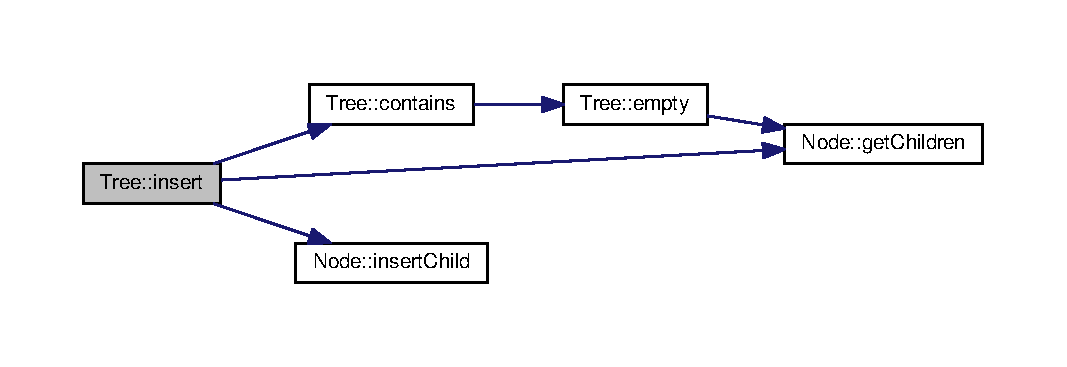
\includegraphics[width=350pt]{class_tree_a0b32b0ca65d8ef7df1dc3a1bd0cf6a99_cgraph}
\end{center}
\end{figure}




Here is the caller graph for this function\-:
\nopagebreak
\begin{figure}[H]
\begin{center}
\leavevmode
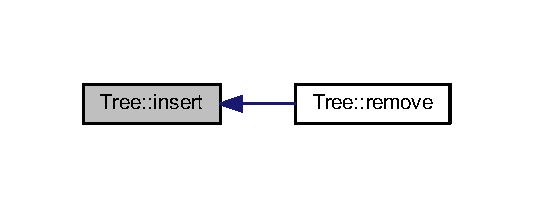
\includegraphics[width=256pt]{class_tree_a0b32b0ca65d8ef7df1dc3a1bd0cf6a99_icgraph}
\end{center}
\end{figure}


\hypertarget{class_tree_a8a64e556c6fc5da582739c3c80d65600}{\index{Tree@{Tree}!leaf\-Info\-To\-File@{leaf\-Info\-To\-File}}
\index{leaf\-Info\-To\-File@{leaf\-Info\-To\-File}!Tree@{Tree}}
\subsubsection[{leaf\-Info\-To\-File}]{\setlength{\rightskip}{0pt plus 5cm}void Tree\-::leaf\-Info\-To\-File (
\begin{DoxyParamCaption}
\item[{int $\ast$}]{in\-Array, }
\item[{int}]{size}
\end{DoxyParamCaption}
)}}\label{class_tree_a8a64e556c6fc5da582739c3c80d65600}


Writes the leaf info to text file. 



Definition at line 356 of file Tree.\-cpp.

\hypertarget{class_tree_a54ddf4e99c00553a6b07cb9b149988e2}{\index{Tree@{Tree}!number\-Of\-Leaves@{number\-Of\-Leaves}}
\index{number\-Of\-Leaves@{number\-Of\-Leaves}!Tree@{Tree}}
\subsubsection[{number\-Of\-Leaves}]{\setlength{\rightskip}{0pt plus 5cm}int Tree\-::number\-Of\-Leaves (
\begin{DoxyParamCaption}
{}
\end{DoxyParamCaption}
)}}\label{class_tree_a54ddf4e99c00553a6b07cb9b149988e2}


Counting the number of leaves that the tree holds with a recursive function. 

\begin{DoxyReturn}{Returns}
Returns the number of leaves contained in the tree 
\end{DoxyReturn}


Definition at line 232 of file Tree.\-cpp.



Here is the call graph for this function\-:
\nopagebreak
\begin{figure}[H]
\begin{center}
\leavevmode
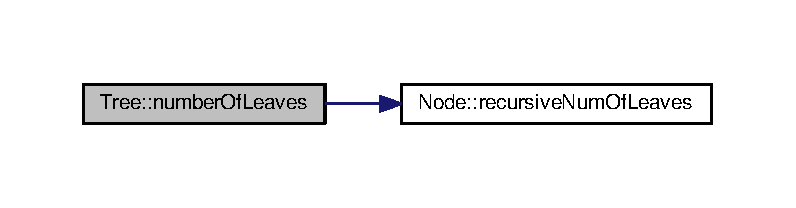
\includegraphics[width=350pt]{class_tree_a54ddf4e99c00553a6b07cb9b149988e2_cgraph}
\end{center}
\end{figure}


\hypertarget{class_tree_a455b10d21349072737b951ad34c2311a}{\index{Tree@{Tree}!number\-Of\-Nodes@{number\-Of\-Nodes}}
\index{number\-Of\-Nodes@{number\-Of\-Nodes}!Tree@{Tree}}
\subsubsection[{number\-Of\-Nodes}]{\setlength{\rightskip}{0pt plus 5cm}int Tree\-::number\-Of\-Nodes (
\begin{DoxyParamCaption}
{}
\end{DoxyParamCaption}
)}}\label{class_tree_a455b10d21349072737b951ad34c2311a}


Counting the number of nodes that the tree holds with a recursive function. 

\begin{DoxyReturn}{Returns}
Returns the number of nodes contained in the tree 
\end{DoxyReturn}


Definition at line 227 of file Tree.\-cpp.



Here is the call graph for this function\-:
\nopagebreak
\begin{figure}[H]
\begin{center}
\leavevmode
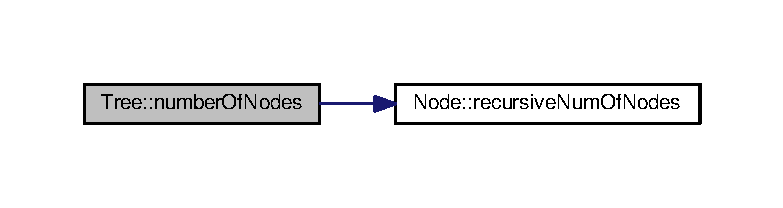
\includegraphics[width=350pt]{class_tree_a455b10d21349072737b951ad34c2311a_cgraph}
\end{center}
\end{figure}


\hypertarget{class_tree_a0015486626ad4da2a7dba4f60ed9aa79}{\index{Tree@{Tree}!remove@{remove}}
\index{remove@{remove}!Tree@{Tree}}
\subsubsection[{remove}]{\setlength{\rightskip}{0pt plus 5cm}void Tree\-::remove (
\begin{DoxyParamCaption}
\item[{int}]{key}
\end{DoxyParamCaption}
)}}\label{class_tree_a0015486626ad4da2a7dba4f60ed9aa79}


Removes the requested leaf while keeping the tree balanced. 


\begin{DoxyParams}{Parameters}
{\em Integer} & value of a leaf to be removed \\
\hline
\end{DoxyParams}


Definition at line 181 of file Tree.\-cpp.



Here is the call graph for this function\-:
\nopagebreak
\begin{figure}[H]
\begin{center}
\leavevmode
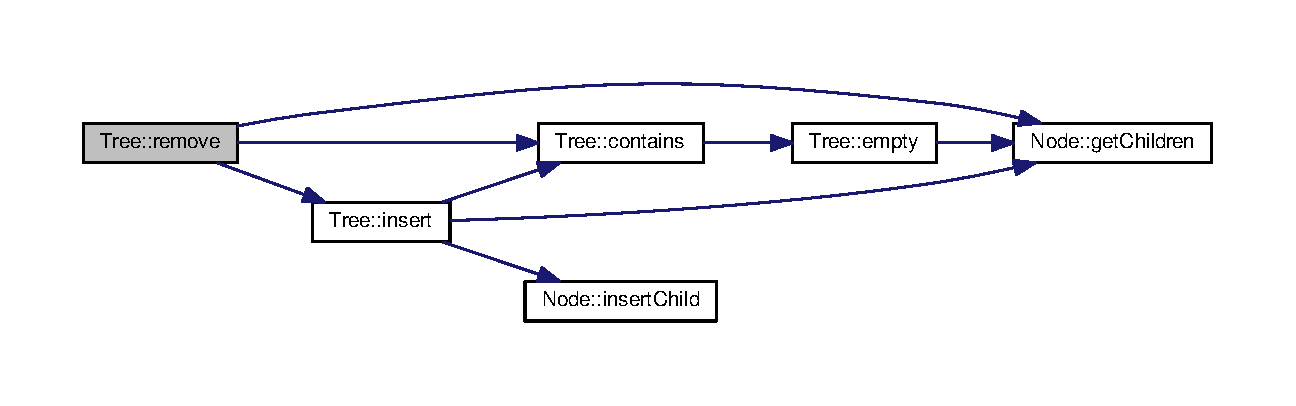
\includegraphics[width=350pt]{class_tree_a0015486626ad4da2a7dba4f60ed9aa79_cgraph}
\end{center}
\end{figure}


\hypertarget{class_tree_a730a56b16e855a1b08a24ee11840d508}{\index{Tree@{Tree}!to\-Int\-Array@{to\-Int\-Array}}
\index{to\-Int\-Array@{to\-Int\-Array}!Tree@{Tree}}
\subsubsection[{to\-Int\-Array}]{\setlength{\rightskip}{0pt plus 5cm}int $\ast$ Tree\-::to\-Int\-Array (
\begin{DoxyParamCaption}
{}
\end{DoxyParamCaption}
)}}\label{class_tree_a730a56b16e855a1b08a24ee11840d508}


An array containing all the info from the leaves. 

\begin{DoxyReturn}{Returns}
Returns an integer array 
\end{DoxyReturn}


Definition at line 237 of file Tree.\-cpp.



Here is the call graph for this function\-:
\nopagebreak
\begin{figure}[H]
\begin{center}
\leavevmode
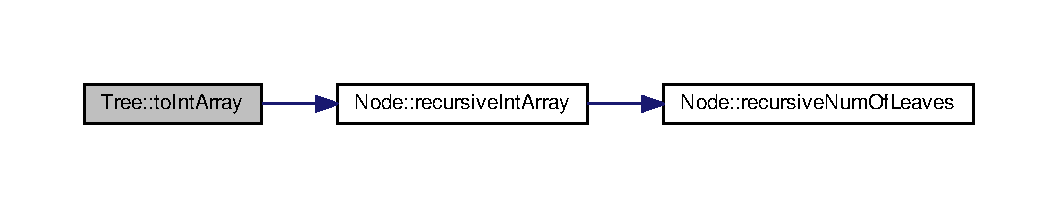
\includegraphics[width=350pt]{class_tree_a730a56b16e855a1b08a24ee11840d508_cgraph}
\end{center}
\end{figure}




\subsection{Member Data Documentation}
\hypertarget{class_tree_ad8e46ce0aead5778cbdd784d1e370d5f}{\index{Tree@{Tree}!root@{root}}
\index{root@{root}!Tree@{Tree}}
\subsubsection[{root}]{\setlength{\rightskip}{0pt plus 5cm}{\bf Node}$\ast$ Tree\-::root}}\label{class_tree_ad8e46ce0aead5778cbdd784d1e370d5f}


Definition at line 94 of file Tree.\-h.



The documentation for this class was generated from the following files\-:\begin{DoxyCompactItemize}
\item 
/home/baios/\-Coding/\-C++/\-Git\-Data\-Structures/\-Data\-Structures/234\-Tree/include/\hyperlink{_tree_8h}{Tree.\-h}\item 
/home/baios/\-Coding/\-C++/\-Git\-Data\-Structures/\-Data\-Structures/234\-Tree/src/\hyperlink{_tree_8cpp}{Tree.\-cpp}\end{DoxyCompactItemize}

\chapter{File Documentation}
\hypertarget{_c_make_c_compiler_id_8c}{\section{/home/baios/\-Desktop/\-Git\-Data\-Structures/\-Data\-Structures/\-Sorting\-And\-Searching/build/\-C\-Make\-Files/2.8.12.2/\-Compiler\-Id\-C/\-C\-Make\-C\-Compiler\-Id.c File Reference}
\label{_c_make_c_compiler_id_8c}\index{/home/baios/\-Desktop/\-Git\-Data\-Structures/\-Data\-Structures/\-Sorting\-And\-Searching/build/\-C\-Make\-Files/2.\-8.\-12.\-2/\-Compiler\-Id\-C/\-C\-Make\-C\-Compiler\-Id.\-c@{/home/baios/\-Desktop/\-Git\-Data\-Structures/\-Data\-Structures/\-Sorting\-And\-Searching/build/\-C\-Make\-Files/2.\-8.\-12.\-2/\-Compiler\-Id\-C/\-C\-Make\-C\-Compiler\-Id.\-c}}
}
\subsection*{Macros}
\begin{DoxyCompactItemize}
\item 
\#define \hyperlink{_c_make_c_compiler_id_8c_a81dee0709ded976b2e0319239f72d174}{C\-O\-M\-P\-I\-L\-E\-R\-\_\-\-I\-D}~\char`\"{}\char`\"{}
\item 
\#define \hyperlink{_c_make_c_compiler_id_8c_adbc5372f40838899018fadbc89bd588b}{P\-L\-A\-T\-F\-O\-R\-M\-\_\-\-I\-D}~\char`\"{}\char`\"{}
\item 
\#define \hyperlink{_c_make_c_compiler_id_8c_aba35d0d200deaeb06aee95ca297acb28}{A\-R\-C\-H\-I\-T\-E\-C\-T\-U\-R\-E\-\_\-\-I\-D}~\char`\"{}\char`\"{}
\item 
\#define \hyperlink{_c_make_c_compiler_id_8c_ad1280362da42492bbc11aa78cbf776ad}{D\-E\-C}(n)
\item 
\#define \hyperlink{_c_make_c_compiler_id_8c_a46d5d95daa1bef867bd0179594310ed5}{H\-E\-X}(n)
\end{DoxyCompactItemize}
\subsection*{Functions}
\begin{DoxyCompactItemize}
\item 
int \hyperlink{_c_make_c_compiler_id_8c_a0ddf1224851353fc92bfbff6f499fa97}{main} (int argc, char $\ast$argv\mbox{[}$\,$\mbox{]})
\end{DoxyCompactItemize}
\subsection*{Variables}
\begin{DoxyCompactItemize}
\item 
char const $\ast$ \hyperlink{_c_make_c_compiler_id_8c_a4b0efeb7a5d59313986b3a0390f050f6}{info\-\_\-compiler} = \char`\"{}I\-N\-F\-O\char`\"{} \char`\"{}\-:\char`\"{} \char`\"{}compiler\mbox{[}\char`\"{} C\-O\-M\-P\-I\-L\-E\-R\-\_\-\-I\-D \char`\"{}\mbox{]}\char`\"{}
\item 
char const $\ast$ \hyperlink{_c_make_c_compiler_id_8c_a2321403dee54ee23f0c2fa849c60f7d4}{info\-\_\-platform} = \char`\"{}I\-N\-F\-O\char`\"{} \char`\"{}\-:\char`\"{} \char`\"{}platform\mbox{[}\char`\"{} P\-L\-A\-T\-F\-O\-R\-M\-\_\-\-I\-D \char`\"{}\mbox{]}\char`\"{}
\item 
char const $\ast$ \hyperlink{_c_make_c_compiler_id_8c_a59647e99d304ed33b15cb284c27ed391}{info\-\_\-arch} = \char`\"{}I\-N\-F\-O\char`\"{} \char`\"{}\-:\char`\"{} \char`\"{}arch\mbox{[}\char`\"{} A\-R\-C\-H\-I\-T\-E\-C\-T\-U\-R\-E\-\_\-\-I\-D \char`\"{}\mbox{]}\char`\"{}
\end{DoxyCompactItemize}


\subsection{Macro Definition Documentation}
\hypertarget{_c_make_c_compiler_id_8c_aba35d0d200deaeb06aee95ca297acb28}{\index{C\-Make\-C\-Compiler\-Id.\-c@{C\-Make\-C\-Compiler\-Id.\-c}!A\-R\-C\-H\-I\-T\-E\-C\-T\-U\-R\-E\-\_\-\-I\-D@{A\-R\-C\-H\-I\-T\-E\-C\-T\-U\-R\-E\-\_\-\-I\-D}}
\index{A\-R\-C\-H\-I\-T\-E\-C\-T\-U\-R\-E\-\_\-\-I\-D@{A\-R\-C\-H\-I\-T\-E\-C\-T\-U\-R\-E\-\_\-\-I\-D}!CMakeCCompilerId.c@{C\-Make\-C\-Compiler\-Id.\-c}}
\subsubsection[{A\-R\-C\-H\-I\-T\-E\-C\-T\-U\-R\-E\-\_\-\-I\-D}]{\setlength{\rightskip}{0pt plus 5cm}\#define A\-R\-C\-H\-I\-T\-E\-C\-T\-U\-R\-E\-\_\-\-I\-D~\char`\"{}\char`\"{}}}\label{_c_make_c_compiler_id_8c_aba35d0d200deaeb06aee95ca297acb28}


Definition at line 320 of file C\-Make\-C\-Compiler\-Id.\-c.

\hypertarget{_c_make_c_compiler_id_8c_a81dee0709ded976b2e0319239f72d174}{\index{C\-Make\-C\-Compiler\-Id.\-c@{C\-Make\-C\-Compiler\-Id.\-c}!C\-O\-M\-P\-I\-L\-E\-R\-\_\-\-I\-D@{C\-O\-M\-P\-I\-L\-E\-R\-\_\-\-I\-D}}
\index{C\-O\-M\-P\-I\-L\-E\-R\-\_\-\-I\-D@{C\-O\-M\-P\-I\-L\-E\-R\-\_\-\-I\-D}!CMakeCCompilerId.c@{C\-Make\-C\-Compiler\-Id.\-c}}
\subsubsection[{C\-O\-M\-P\-I\-L\-E\-R\-\_\-\-I\-D}]{\setlength{\rightskip}{0pt plus 5cm}\#define C\-O\-M\-P\-I\-L\-E\-R\-\_\-\-I\-D~\char`\"{}\char`\"{}}}\label{_c_make_c_compiler_id_8c_a81dee0709ded976b2e0319239f72d174}


Definition at line 200 of file C\-Make\-C\-Compiler\-Id.\-c.

\hypertarget{_c_make_c_compiler_id_8c_ad1280362da42492bbc11aa78cbf776ad}{\index{C\-Make\-C\-Compiler\-Id.\-c@{C\-Make\-C\-Compiler\-Id.\-c}!D\-E\-C@{D\-E\-C}}
\index{D\-E\-C@{D\-E\-C}!CMakeCCompilerId.c@{C\-Make\-C\-Compiler\-Id.\-c}}
\subsubsection[{D\-E\-C}]{\setlength{\rightskip}{0pt plus 5cm}\#define D\-E\-C(
\begin{DoxyParamCaption}
\item[{}]{n}
\end{DoxyParamCaption}
)}}\label{_c_make_c_compiler_id_8c_ad1280362da42492bbc11aa78cbf776ad}
{\bfseries Value\-:}
\begin{DoxyCode}
(\textcolor{charliteral}{'0'} + (((n) / 10000000)%10)), \(\backslash\)
  (\textcolor{charliteral}{'0'} + (((n) / 1000000)%10)),  \(\backslash\)
  (\textcolor{charliteral}{'0'} + (((n) / 100000)%10)),   \(\backslash\)
  (\textcolor{charliteral}{'0'} + (((n) / 10000)%10)),    \(\backslash\)
  (\textcolor{charliteral}{'0'} + (((n) / 1000)%10)),     \(\backslash\)
  (\textcolor{charliteral}{'0'} + (((n) / 100)%10)),      \(\backslash\)
  (\textcolor{charliteral}{'0'} + (((n) / 10)%10)),       \(\backslash\)
  (\textcolor{charliteral}{'0'} +  ((n) % 10))
\end{DoxyCode}


Definition at line 324 of file C\-Make\-C\-Compiler\-Id.\-c.

\hypertarget{_c_make_c_compiler_id_8c_a46d5d95daa1bef867bd0179594310ed5}{\index{C\-Make\-C\-Compiler\-Id.\-c@{C\-Make\-C\-Compiler\-Id.\-c}!H\-E\-X@{H\-E\-X}}
\index{H\-E\-X@{H\-E\-X}!CMakeCCompilerId.c@{C\-Make\-C\-Compiler\-Id.\-c}}
\subsubsection[{H\-E\-X}]{\setlength{\rightskip}{0pt plus 5cm}\#define H\-E\-X(
\begin{DoxyParamCaption}
\item[{}]{n}
\end{DoxyParamCaption}
)}}\label{_c_make_c_compiler_id_8c_a46d5d95daa1bef867bd0179594310ed5}
{\bfseries Value\-:}
\begin{DoxyCode}
(\textcolor{charliteral}{'0'} + ((n)>>28 & 0xF)), \(\backslash\)
  (\textcolor{charliteral}{'0'} + ((n)>>24 & 0xF)), \(\backslash\)
  (\textcolor{charliteral}{'0'} + ((n)>>20 & 0xF)), \(\backslash\)
  (\textcolor{charliteral}{'0'} + ((n)>>16 & 0xF)), \(\backslash\)
  (\textcolor{charliteral}{'0'} + ((n)>>12 & 0xF)), \(\backslash\)
  (\textcolor{charliteral}{'0'} + ((n)>>8  & 0xF)), \(\backslash\)
  (\textcolor{charliteral}{'0'} + ((n)>>4  & 0xF)), \(\backslash\)
  (\textcolor{charliteral}{'0'} + ((n)     & 0xF))
\end{DoxyCode}


Definition at line 335 of file C\-Make\-C\-Compiler\-Id.\-c.

\hypertarget{_c_make_c_compiler_id_8c_adbc5372f40838899018fadbc89bd588b}{\index{C\-Make\-C\-Compiler\-Id.\-c@{C\-Make\-C\-Compiler\-Id.\-c}!P\-L\-A\-T\-F\-O\-R\-M\-\_\-\-I\-D@{P\-L\-A\-T\-F\-O\-R\-M\-\_\-\-I\-D}}
\index{P\-L\-A\-T\-F\-O\-R\-M\-\_\-\-I\-D@{P\-L\-A\-T\-F\-O\-R\-M\-\_\-\-I\-D}!CMakeCCompilerId.c@{C\-Make\-C\-Compiler\-Id.\-c}}
\subsubsection[{P\-L\-A\-T\-F\-O\-R\-M\-\_\-\-I\-D}]{\setlength{\rightskip}{0pt plus 5cm}\#define P\-L\-A\-T\-F\-O\-R\-M\-\_\-\-I\-D~\char`\"{}\char`\"{}}}\label{_c_make_c_compiler_id_8c_adbc5372f40838899018fadbc89bd588b}


Definition at line 287 of file C\-Make\-C\-Compiler\-Id.\-c.



\subsection{Function Documentation}
\hypertarget{_c_make_c_compiler_id_8c_a0ddf1224851353fc92bfbff6f499fa97}{\index{C\-Make\-C\-Compiler\-Id.\-c@{C\-Make\-C\-Compiler\-Id.\-c}!main@{main}}
\index{main@{main}!CMakeCCompilerId.c@{C\-Make\-C\-Compiler\-Id.\-c}}
\subsubsection[{main}]{\setlength{\rightskip}{0pt plus 5cm}int main (
\begin{DoxyParamCaption}
\item[{int}]{argc, }
\item[{char $\ast$}]{argv\mbox{[}$\,$\mbox{]}}
\end{DoxyParamCaption}
)}}\label{_c_make_c_compiler_id_8c_a0ddf1224851353fc92bfbff6f499fa97}


Definition at line 377 of file C\-Make\-C\-Compiler\-Id.\-c.



\subsection{Variable Documentation}
\hypertarget{_c_make_c_compiler_id_8c_a59647e99d304ed33b15cb284c27ed391}{\index{C\-Make\-C\-Compiler\-Id.\-c@{C\-Make\-C\-Compiler\-Id.\-c}!info\-\_\-arch@{info\-\_\-arch}}
\index{info\-\_\-arch@{info\-\_\-arch}!CMakeCCompilerId.c@{C\-Make\-C\-Compiler\-Id.\-c}}
\subsubsection[{info\-\_\-arch}]{\setlength{\rightskip}{0pt plus 5cm}char const$\ast$ info\-\_\-arch = \char`\"{}I\-N\-F\-O\char`\"{} \char`\"{}\-:\char`\"{} \char`\"{}arch\mbox{[}\char`\"{} A\-R\-C\-H\-I\-T\-E\-C\-T\-U\-R\-E\-\_\-\-I\-D \char`\"{}\mbox{]}\char`\"{}}}\label{_c_make_c_compiler_id_8c_a59647e99d304ed33b15cb284c27ed391}


Definition at line 368 of file C\-Make\-C\-Compiler\-Id.\-c.

\hypertarget{_c_make_c_compiler_id_8c_a4b0efeb7a5d59313986b3a0390f050f6}{\index{C\-Make\-C\-Compiler\-Id.\-c@{C\-Make\-C\-Compiler\-Id.\-c}!info\-\_\-compiler@{info\-\_\-compiler}}
\index{info\-\_\-compiler@{info\-\_\-compiler}!CMakeCCompilerId.c@{C\-Make\-C\-Compiler\-Id.\-c}}
\subsubsection[{info\-\_\-compiler}]{\setlength{\rightskip}{0pt plus 5cm}char const$\ast$ info\-\_\-compiler = \char`\"{}I\-N\-F\-O\char`\"{} \char`\"{}\-:\char`\"{} \char`\"{}compiler\mbox{[}\char`\"{} C\-O\-M\-P\-I\-L\-E\-R\-\_\-\-I\-D \char`\"{}\mbox{]}\char`\"{}}}\label{_c_make_c_compiler_id_8c_a4b0efeb7a5d59313986b3a0390f050f6}


Definition at line 208 of file C\-Make\-C\-Compiler\-Id.\-c.

\hypertarget{_c_make_c_compiler_id_8c_a2321403dee54ee23f0c2fa849c60f7d4}{\index{C\-Make\-C\-Compiler\-Id.\-c@{C\-Make\-C\-Compiler\-Id.\-c}!info\-\_\-platform@{info\-\_\-platform}}
\index{info\-\_\-platform@{info\-\_\-platform}!CMakeCCompilerId.c@{C\-Make\-C\-Compiler\-Id.\-c}}
\subsubsection[{info\-\_\-platform}]{\setlength{\rightskip}{0pt plus 5cm}char const$\ast$ info\-\_\-platform = \char`\"{}I\-N\-F\-O\char`\"{} \char`\"{}\-:\char`\"{} \char`\"{}platform\mbox{[}\char`\"{} P\-L\-A\-T\-F\-O\-R\-M\-\_\-\-I\-D \char`\"{}\mbox{]}\char`\"{}}}\label{_c_make_c_compiler_id_8c_a2321403dee54ee23f0c2fa849c60f7d4}


Definition at line 367 of file C\-Make\-C\-Compiler\-Id.\-c.


\hypertarget{_c_make_c_x_x_compiler_id_8cpp}{\section{/home/baios/\-Coding/\-C++/\-Git\-Data\-Structures/\-Data\-Structures/234\-Tree/build/\-C\-Make\-Files/2.8.12.2/\-Compiler\-Id\-C\-X\-X/\-C\-Make\-C\-X\-X\-Compiler\-Id.cpp File Reference}
\label{_c_make_c_x_x_compiler_id_8cpp}\index{/home/baios/\-Coding/\-C++/\-Git\-Data\-Structures/\-Data\-Structures/234\-Tree/build/\-C\-Make\-Files/2.\-8.\-12.\-2/\-Compiler\-Id\-C\-X\-X/\-C\-Make\-C\-X\-X\-Compiler\-Id.\-cpp@{/home/baios/\-Coding/\-C++/\-Git\-Data\-Structures/\-Data\-Structures/234\-Tree/build/\-C\-Make\-Files/2.\-8.\-12.\-2/\-Compiler\-Id\-C\-X\-X/\-C\-Make\-C\-X\-X\-Compiler\-Id.\-cpp}}
}
\subsection*{Macros}
\begin{DoxyCompactItemize}
\item 
\#define \hyperlink{_c_make_c_x_x_compiler_id_8cpp_a81dee0709ded976b2e0319239f72d174}{C\-O\-M\-P\-I\-L\-E\-R\-\_\-\-I\-D}~\char`\"{}\char`\"{}
\item 
\#define \hyperlink{_c_make_c_x_x_compiler_id_8cpp_adbc5372f40838899018fadbc89bd588b}{P\-L\-A\-T\-F\-O\-R\-M\-\_\-\-I\-D}~\char`\"{}\char`\"{}
\item 
\#define \hyperlink{_c_make_c_x_x_compiler_id_8cpp_aba35d0d200deaeb06aee95ca297acb28}{A\-R\-C\-H\-I\-T\-E\-C\-T\-U\-R\-E\-\_\-\-I\-D}~\char`\"{}\char`\"{}
\item 
\#define \hyperlink{_c_make_c_x_x_compiler_id_8cpp_ad1280362da42492bbc11aa78cbf776ad}{D\-E\-C}(n)
\item 
\#define \hyperlink{_c_make_c_x_x_compiler_id_8cpp_a46d5d95daa1bef867bd0179594310ed5}{H\-E\-X}(n)
\end{DoxyCompactItemize}
\subsection*{Functions}
\begin{DoxyCompactItemize}
\item 
int \hyperlink{_c_make_c_x_x_compiler_id_8cpp_a0ddf1224851353fc92bfbff6f499fa97}{main} (int argc, char $\ast$argv\mbox{[}$\,$\mbox{]})
\end{DoxyCompactItemize}
\subsection*{Variables}
\begin{DoxyCompactItemize}
\item 
char const $\ast$ \hyperlink{_c_make_c_x_x_compiler_id_8cpp_a4b0efeb7a5d59313986b3a0390f050f6}{info\-\_\-compiler} = \char`\"{}I\-N\-F\-O\char`\"{} \char`\"{}\-:\char`\"{} \char`\"{}compiler\mbox{[}\char`\"{} C\-O\-M\-P\-I\-L\-E\-R\-\_\-\-I\-D \char`\"{}\mbox{]}\char`\"{}
\item 
char const $\ast$ \hyperlink{_c_make_c_x_x_compiler_id_8cpp_a2321403dee54ee23f0c2fa849c60f7d4}{info\-\_\-platform} = \char`\"{}I\-N\-F\-O\char`\"{} \char`\"{}\-:\char`\"{} \char`\"{}platform\mbox{[}\char`\"{} P\-L\-A\-T\-F\-O\-R\-M\-\_\-\-I\-D \char`\"{}\mbox{]}\char`\"{}
\item 
char const $\ast$ \hyperlink{_c_make_c_x_x_compiler_id_8cpp_a59647e99d304ed33b15cb284c27ed391}{info\-\_\-arch} = \char`\"{}I\-N\-F\-O\char`\"{} \char`\"{}\-:\char`\"{} \char`\"{}arch\mbox{[}\char`\"{} A\-R\-C\-H\-I\-T\-E\-C\-T\-U\-R\-E\-\_\-\-I\-D \char`\"{}\mbox{]}\char`\"{}
\end{DoxyCompactItemize}


\subsection{Macro Definition Documentation}
\hypertarget{_c_make_c_x_x_compiler_id_8cpp_aba35d0d200deaeb06aee95ca297acb28}{\index{C\-Make\-C\-X\-X\-Compiler\-Id.\-cpp@{C\-Make\-C\-X\-X\-Compiler\-Id.\-cpp}!A\-R\-C\-H\-I\-T\-E\-C\-T\-U\-R\-E\-\_\-\-I\-D@{A\-R\-C\-H\-I\-T\-E\-C\-T\-U\-R\-E\-\_\-\-I\-D}}
\index{A\-R\-C\-H\-I\-T\-E\-C\-T\-U\-R\-E\-\_\-\-I\-D@{A\-R\-C\-H\-I\-T\-E\-C\-T\-U\-R\-E\-\_\-\-I\-D}!CMakeCXXCompilerId.cpp@{C\-Make\-C\-X\-X\-Compiler\-Id.\-cpp}}
\subsubsection[{A\-R\-C\-H\-I\-T\-E\-C\-T\-U\-R\-E\-\_\-\-I\-D}]{\setlength{\rightskip}{0pt plus 5cm}\#define A\-R\-C\-H\-I\-T\-E\-C\-T\-U\-R\-E\-\_\-\-I\-D~\char`\"{}\char`\"{}}}\label{_c_make_c_x_x_compiler_id_8cpp_aba35d0d200deaeb06aee95ca297acb28}


Definition at line 313 of file C\-Make\-C\-X\-X\-Compiler\-Id.\-cpp.

\hypertarget{_c_make_c_x_x_compiler_id_8cpp_a81dee0709ded976b2e0319239f72d174}{\index{C\-Make\-C\-X\-X\-Compiler\-Id.\-cpp@{C\-Make\-C\-X\-X\-Compiler\-Id.\-cpp}!C\-O\-M\-P\-I\-L\-E\-R\-\_\-\-I\-D@{C\-O\-M\-P\-I\-L\-E\-R\-\_\-\-I\-D}}
\index{C\-O\-M\-P\-I\-L\-E\-R\-\_\-\-I\-D@{C\-O\-M\-P\-I\-L\-E\-R\-\_\-\-I\-D}!CMakeCXXCompilerId.cpp@{C\-Make\-C\-X\-X\-Compiler\-Id.\-cpp}}
\subsubsection[{C\-O\-M\-P\-I\-L\-E\-R\-\_\-\-I\-D}]{\setlength{\rightskip}{0pt plus 5cm}\#define C\-O\-M\-P\-I\-L\-E\-R\-\_\-\-I\-D~\char`\"{}\char`\"{}}}\label{_c_make_c_x_x_compiler_id_8cpp_a81dee0709ded976b2e0319239f72d174}


Definition at line 193 of file C\-Make\-C\-X\-X\-Compiler\-Id.\-cpp.

\hypertarget{_c_make_c_x_x_compiler_id_8cpp_ad1280362da42492bbc11aa78cbf776ad}{\index{C\-Make\-C\-X\-X\-Compiler\-Id.\-cpp@{C\-Make\-C\-X\-X\-Compiler\-Id.\-cpp}!D\-E\-C@{D\-E\-C}}
\index{D\-E\-C@{D\-E\-C}!CMakeCXXCompilerId.cpp@{C\-Make\-C\-X\-X\-Compiler\-Id.\-cpp}}
\subsubsection[{D\-E\-C}]{\setlength{\rightskip}{0pt plus 5cm}\#define D\-E\-C(
\begin{DoxyParamCaption}
\item[{}]{n}
\end{DoxyParamCaption}
)}}\label{_c_make_c_x_x_compiler_id_8cpp_ad1280362da42492bbc11aa78cbf776ad}
{\bfseries Value\-:}
\begin{DoxyCode}
(\textcolor{charliteral}{'0'} + (((n) / 10000000)%10)), \(\backslash\)
  (\textcolor{charliteral}{'0'} + (((n) / 1000000)%10)),  \(\backslash\)
  (\textcolor{charliteral}{'0'} + (((n) / 100000)%10)),   \(\backslash\)
  (\textcolor{charliteral}{'0'} + (((n) / 10000)%10)),    \(\backslash\)
  (\textcolor{charliteral}{'0'} + (((n) / 1000)%10)),     \(\backslash\)
  (\textcolor{charliteral}{'0'} + (((n) / 100)%10)),      \(\backslash\)
  (\textcolor{charliteral}{'0'} + (((n) / 10)%10)),       \(\backslash\)
  (\textcolor{charliteral}{'0'} +  ((n) % 10))
\end{DoxyCode}


Definition at line 317 of file C\-Make\-C\-X\-X\-Compiler\-Id.\-cpp.

\hypertarget{_c_make_c_x_x_compiler_id_8cpp_a46d5d95daa1bef867bd0179594310ed5}{\index{C\-Make\-C\-X\-X\-Compiler\-Id.\-cpp@{C\-Make\-C\-X\-X\-Compiler\-Id.\-cpp}!H\-E\-X@{H\-E\-X}}
\index{H\-E\-X@{H\-E\-X}!CMakeCXXCompilerId.cpp@{C\-Make\-C\-X\-X\-Compiler\-Id.\-cpp}}
\subsubsection[{H\-E\-X}]{\setlength{\rightskip}{0pt plus 5cm}\#define H\-E\-X(
\begin{DoxyParamCaption}
\item[{}]{n}
\end{DoxyParamCaption}
)}}\label{_c_make_c_x_x_compiler_id_8cpp_a46d5d95daa1bef867bd0179594310ed5}
{\bfseries Value\-:}
\begin{DoxyCode}
(\textcolor{charliteral}{'0'} + ((n)>>28 & 0xF)), \(\backslash\)
  (\textcolor{charliteral}{'0'} + ((n)>>24 & 0xF)), \(\backslash\)
  (\textcolor{charliteral}{'0'} + ((n)>>20 & 0xF)), \(\backslash\)
  (\textcolor{charliteral}{'0'} + ((n)>>16 & 0xF)), \(\backslash\)
  (\textcolor{charliteral}{'0'} + ((n)>>12 & 0xF)), \(\backslash\)
  (\textcolor{charliteral}{'0'} + ((n)>>8  & 0xF)), \(\backslash\)
  (\textcolor{charliteral}{'0'} + ((n)>>4  & 0xF)), \(\backslash\)
  (\textcolor{charliteral}{'0'} + ((n)     & 0xF))
\end{DoxyCode}


Definition at line 328 of file C\-Make\-C\-X\-X\-Compiler\-Id.\-cpp.

\hypertarget{_c_make_c_x_x_compiler_id_8cpp_adbc5372f40838899018fadbc89bd588b}{\index{C\-Make\-C\-X\-X\-Compiler\-Id.\-cpp@{C\-Make\-C\-X\-X\-Compiler\-Id.\-cpp}!P\-L\-A\-T\-F\-O\-R\-M\-\_\-\-I\-D@{P\-L\-A\-T\-F\-O\-R\-M\-\_\-\-I\-D}}
\index{P\-L\-A\-T\-F\-O\-R\-M\-\_\-\-I\-D@{P\-L\-A\-T\-F\-O\-R\-M\-\_\-\-I\-D}!CMakeCXXCompilerId.cpp@{C\-Make\-C\-X\-X\-Compiler\-Id.\-cpp}}
\subsubsection[{P\-L\-A\-T\-F\-O\-R\-M\-\_\-\-I\-D}]{\setlength{\rightskip}{0pt plus 5cm}\#define P\-L\-A\-T\-F\-O\-R\-M\-\_\-\-I\-D~\char`\"{}\char`\"{}}}\label{_c_make_c_x_x_compiler_id_8cpp_adbc5372f40838899018fadbc89bd588b}


Definition at line 280 of file C\-Make\-C\-X\-X\-Compiler\-Id.\-cpp.



\subsection{Function Documentation}
\hypertarget{_c_make_c_x_x_compiler_id_8cpp_a0ddf1224851353fc92bfbff6f499fa97}{\index{C\-Make\-C\-X\-X\-Compiler\-Id.\-cpp@{C\-Make\-C\-X\-X\-Compiler\-Id.\-cpp}!main@{main}}
\index{main@{main}!CMakeCXXCompilerId.cpp@{C\-Make\-C\-X\-X\-Compiler\-Id.\-cpp}}
\subsubsection[{main}]{\setlength{\rightskip}{0pt plus 5cm}int main (
\begin{DoxyParamCaption}
\item[{int}]{argc, }
\item[{char $\ast$}]{argv\mbox{[}$\,$\mbox{]}}
\end{DoxyParamCaption}
)}}\label{_c_make_c_x_x_compiler_id_8cpp_a0ddf1224851353fc92bfbff6f499fa97}


Definition at line 367 of file C\-Make\-C\-X\-X\-Compiler\-Id.\-cpp.



\subsection{Variable Documentation}
\hypertarget{_c_make_c_x_x_compiler_id_8cpp_a59647e99d304ed33b15cb284c27ed391}{\index{C\-Make\-C\-X\-X\-Compiler\-Id.\-cpp@{C\-Make\-C\-X\-X\-Compiler\-Id.\-cpp}!info\-\_\-arch@{info\-\_\-arch}}
\index{info\-\_\-arch@{info\-\_\-arch}!CMakeCXXCompilerId.cpp@{C\-Make\-C\-X\-X\-Compiler\-Id.\-cpp}}
\subsubsection[{info\-\_\-arch}]{\setlength{\rightskip}{0pt plus 5cm}char const$\ast$ info\-\_\-arch = \char`\"{}I\-N\-F\-O\char`\"{} \char`\"{}\-:\char`\"{} \char`\"{}arch\mbox{[}\char`\"{} A\-R\-C\-H\-I\-T\-E\-C\-T\-U\-R\-E\-\_\-\-I\-D \char`\"{}\mbox{]}\char`\"{}}}\label{_c_make_c_x_x_compiler_id_8cpp_a59647e99d304ed33b15cb284c27ed391}


Definition at line 361 of file C\-Make\-C\-X\-X\-Compiler\-Id.\-cpp.

\hypertarget{_c_make_c_x_x_compiler_id_8cpp_a4b0efeb7a5d59313986b3a0390f050f6}{\index{C\-Make\-C\-X\-X\-Compiler\-Id.\-cpp@{C\-Make\-C\-X\-X\-Compiler\-Id.\-cpp}!info\-\_\-compiler@{info\-\_\-compiler}}
\index{info\-\_\-compiler@{info\-\_\-compiler}!CMakeCXXCompilerId.cpp@{C\-Make\-C\-X\-X\-Compiler\-Id.\-cpp}}
\subsubsection[{info\-\_\-compiler}]{\setlength{\rightskip}{0pt plus 5cm}char const$\ast$ info\-\_\-compiler = \char`\"{}I\-N\-F\-O\char`\"{} \char`\"{}\-:\char`\"{} \char`\"{}compiler\mbox{[}\char`\"{} C\-O\-M\-P\-I\-L\-E\-R\-\_\-\-I\-D \char`\"{}\mbox{]}\char`\"{}}}\label{_c_make_c_x_x_compiler_id_8cpp_a4b0efeb7a5d59313986b3a0390f050f6}


Definition at line 201 of file C\-Make\-C\-X\-X\-Compiler\-Id.\-cpp.

\hypertarget{_c_make_c_x_x_compiler_id_8cpp_a2321403dee54ee23f0c2fa849c60f7d4}{\index{C\-Make\-C\-X\-X\-Compiler\-Id.\-cpp@{C\-Make\-C\-X\-X\-Compiler\-Id.\-cpp}!info\-\_\-platform@{info\-\_\-platform}}
\index{info\-\_\-platform@{info\-\_\-platform}!CMakeCXXCompilerId.cpp@{C\-Make\-C\-X\-X\-Compiler\-Id.\-cpp}}
\subsubsection[{info\-\_\-platform}]{\setlength{\rightskip}{0pt plus 5cm}char const$\ast$ info\-\_\-platform = \char`\"{}I\-N\-F\-O\char`\"{} \char`\"{}\-:\char`\"{} \char`\"{}platform\mbox{[}\char`\"{} P\-L\-A\-T\-F\-O\-R\-M\-\_\-\-I\-D \char`\"{}\mbox{]}\char`\"{}}}\label{_c_make_c_x_x_compiler_id_8cpp_a2321403dee54ee23f0c2fa849c60f7d4}


Definition at line 360 of file C\-Make\-C\-X\-X\-Compiler\-Id.\-cpp.


\hypertarget{_graph_vis_8h}{\section{/home/baios/\-Coding/\-C++/\-Git\-Data\-Structures/\-Data\-Structures/234\-Tree/include/\-Graph\-Vis.h File Reference}
\label{_graph_vis_8h}\index{/home/baios/\-Coding/\-C++/\-Git\-Data\-Structures/\-Data\-Structures/234\-Tree/include/\-Graph\-Vis.\-h@{/home/baios/\-Coding/\-C++/\-Git\-Data\-Structures/\-Data\-Structures/234\-Tree/include/\-Graph\-Vis.\-h}}
}
{\ttfamily \#include $<$graphviz/gvc.\-h$>$}\\*
{\ttfamily \#include $<$graphviz/cgraph.\-h$>$}\\*
{\ttfamily \#include $<$graphviz/graph.\-h$>$}\\*
{\ttfamily \#include $<$string$>$}\\*
{\ttfamily \#include \char`\"{}Tree.\-h\char`\"{}}\\*
Include dependency graph for Graph\-Vis.\-h\-:
\nopagebreak
\begin{figure}[H]
\begin{center}
\leavevmode
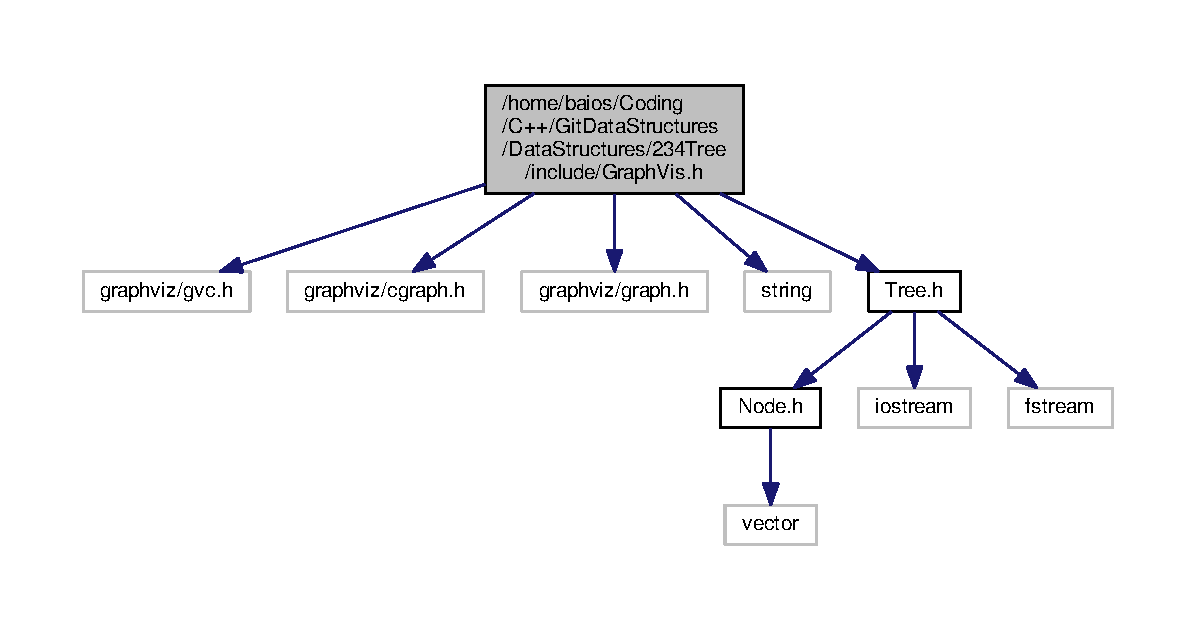
\includegraphics[width=350pt]{_graph_vis_8h__incl}
\end{center}
\end{figure}
This graph shows which files directly or indirectly include this file\-:
\nopagebreak
\begin{figure}[H]
\begin{center}
\leavevmode
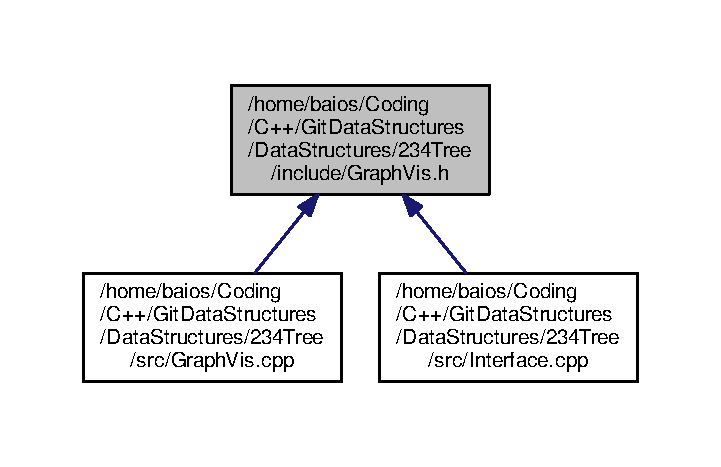
\includegraphics[width=346pt]{_graph_vis_8h__dep__incl}
\end{center}
\end{figure}
\subsection*{Classes}
\begin{DoxyCompactItemize}
\item 
class \hyperlink{class_graph_vis}{Graph\-Vis}
\begin{DoxyCompactList}\small\item\em \hyperlink{class_graph_vis}{Graph\-Vis} Class. \end{DoxyCompactList}\end{DoxyCompactItemize}

\hypertarget{_interface_8h}{\section{/home/baios/\-Coding/\-C++/\-Git\-Data\-Structures/\-Data\-Structures/234\-Tree/include/\-Interface.h File Reference}
\label{_interface_8h}\index{/home/baios/\-Coding/\-C++/\-Git\-Data\-Structures/\-Data\-Structures/234\-Tree/include/\-Interface.\-h@{/home/baios/\-Coding/\-C++/\-Git\-Data\-Structures/\-Data\-Structures/234\-Tree/include/\-Interface.\-h}}
}
{\ttfamily \#include \char`\"{}Tree.\-h\char`\"{}}\\*
Include dependency graph for Interface.\-h\-:
\nopagebreak
\begin{figure}[H]
\begin{center}
\leavevmode
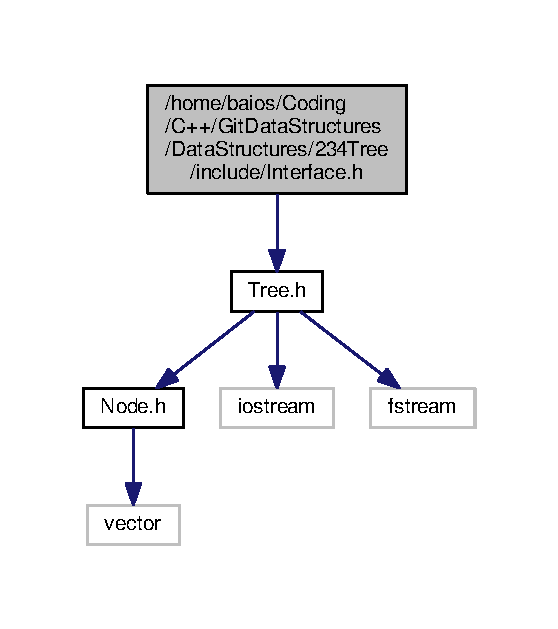
\includegraphics[width=268pt]{_interface_8h__incl}
\end{center}
\end{figure}
This graph shows which files directly or indirectly include this file\-:
\nopagebreak
\begin{figure}[H]
\begin{center}
\leavevmode
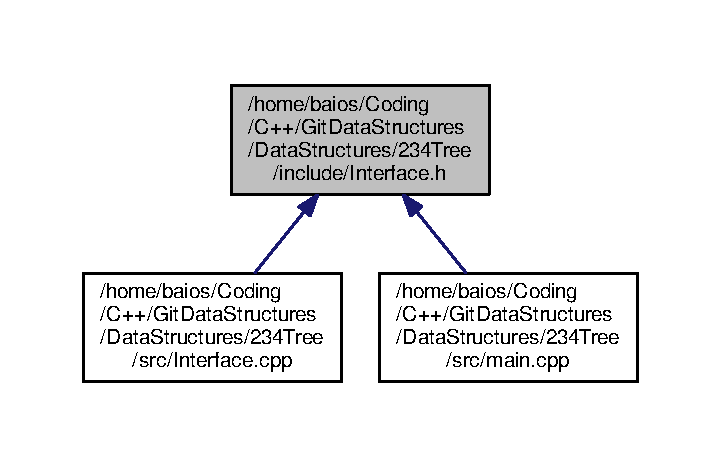
\includegraphics[width=346pt]{_interface_8h__dep__incl}
\end{center}
\end{figure}
\subsection*{Classes}
\begin{DoxyCompactItemize}
\item 
class \hyperlink{class_interface}{Interface}
\begin{DoxyCompactList}\small\item\em \hyperlink{class_interface}{Interface} Class. \end{DoxyCompactList}\end{DoxyCompactItemize}

\hypertarget{_node_8h}{\section{/home/baios/\-Coding/\-C++/\-Git\-Data\-Structures/\-Data\-Structures/234\-Tree/include/\-Node.h File Reference}
\label{_node_8h}\index{/home/baios/\-Coding/\-C++/\-Git\-Data\-Structures/\-Data\-Structures/234\-Tree/include/\-Node.\-h@{/home/baios/\-Coding/\-C++/\-Git\-Data\-Structures/\-Data\-Structures/234\-Tree/include/\-Node.\-h}}
}
{\ttfamily \#include $<$vector$>$}\\*
Include dependency graph for Node.\-h\-:
\nopagebreak
\begin{figure}[H]
\begin{center}
\leavevmode
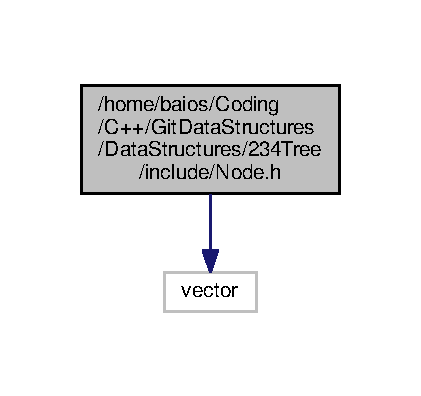
\includegraphics[width=202pt]{_node_8h__incl}
\end{center}
\end{figure}
This graph shows which files directly or indirectly include this file\-:
\nopagebreak
\begin{figure}[H]
\begin{center}
\leavevmode
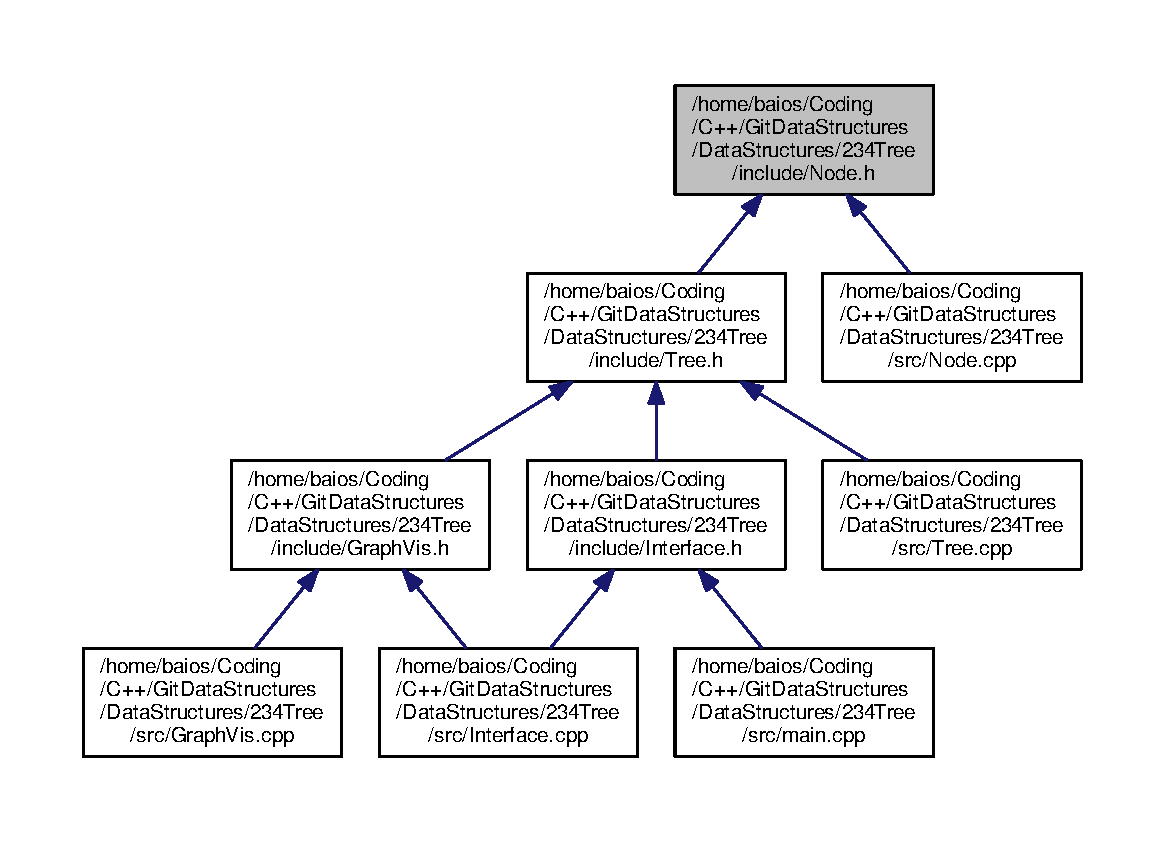
\includegraphics[width=350pt]{_node_8h__dep__incl}
\end{center}
\end{figure}
\subsection*{Classes}
\begin{DoxyCompactItemize}
\item 
class \hyperlink{class_node}{Node}
\begin{DoxyCompactList}\small\item\em \hyperlink{class_node}{Node} Class. \end{DoxyCompactList}\end{DoxyCompactItemize}

\hypertarget{_tree_8h}{\section{/home/baios/\-Coding/\-C++/\-Git\-Data\-Structures/\-Data\-Structures/234\-Tree/include/\-Tree.h File Reference}
\label{_tree_8h}\index{/home/baios/\-Coding/\-C++/\-Git\-Data\-Structures/\-Data\-Structures/234\-Tree/include/\-Tree.\-h@{/home/baios/\-Coding/\-C++/\-Git\-Data\-Structures/\-Data\-Structures/234\-Tree/include/\-Tree.\-h}}
}
{\ttfamily \#include \char`\"{}Node.\-h\char`\"{}}\\*
{\ttfamily \#include $<$iostream$>$}\\*
{\ttfamily \#include $<$fstream$>$}\\*
Include dependency graph for Tree.\-h\-:
\nopagebreak
\begin{figure}[H]
\begin{center}
\leavevmode
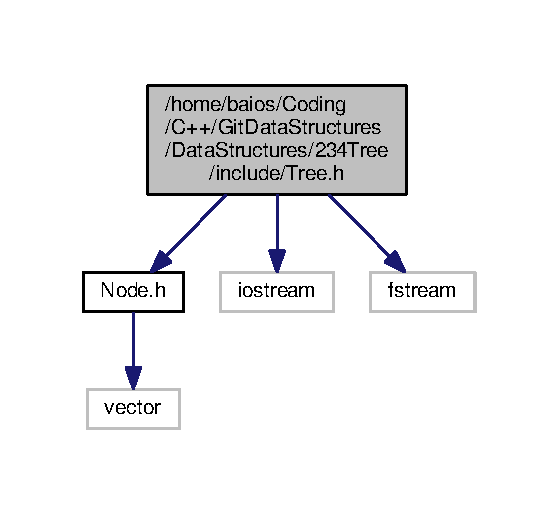
\includegraphics[width=268pt]{_tree_8h__incl}
\end{center}
\end{figure}
This graph shows which files directly or indirectly include this file\-:
\nopagebreak
\begin{figure}[H]
\begin{center}
\leavevmode
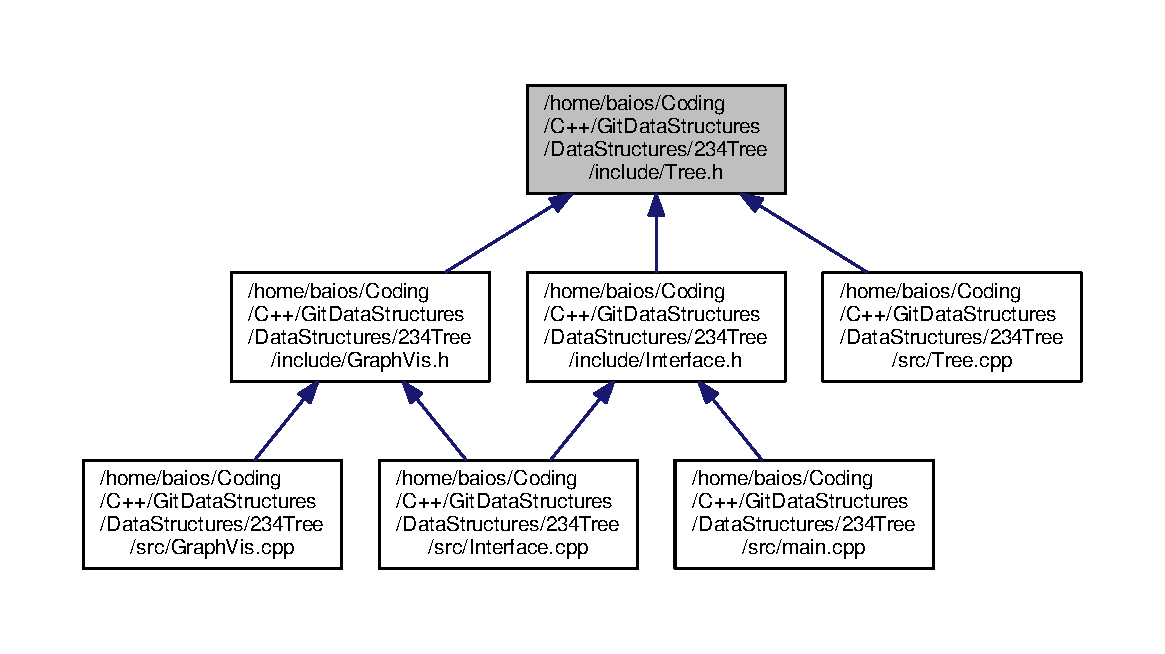
\includegraphics[width=350pt]{_tree_8h__dep__incl}
\end{center}
\end{figure}
\subsection*{Classes}
\begin{DoxyCompactItemize}
\item 
class \hyperlink{class_tree}{Tree}
\begin{DoxyCompactList}\small\item\em \hyperlink{class_tree}{Tree} Class. \end{DoxyCompactList}\end{DoxyCompactItemize}

\hypertarget{_graph_vis_8cpp}{\section{/home/baios/\-Coding/\-C++/\-Git\-Data\-Structures/\-Data\-Structures/234\-Tree/src/\-Graph\-Vis.cpp File Reference}
\label{_graph_vis_8cpp}\index{/home/baios/\-Coding/\-C++/\-Git\-Data\-Structures/\-Data\-Structures/234\-Tree/src/\-Graph\-Vis.\-cpp@{/home/baios/\-Coding/\-C++/\-Git\-Data\-Structures/\-Data\-Structures/234\-Tree/src/\-Graph\-Vis.\-cpp}}
}
{\ttfamily \#include \char`\"{}Graph\-Vis.\-h\char`\"{}}\\*
Include dependency graph for Graph\-Vis.\-cpp\-:
\nopagebreak
\begin{figure}[H]
\begin{center}
\leavevmode
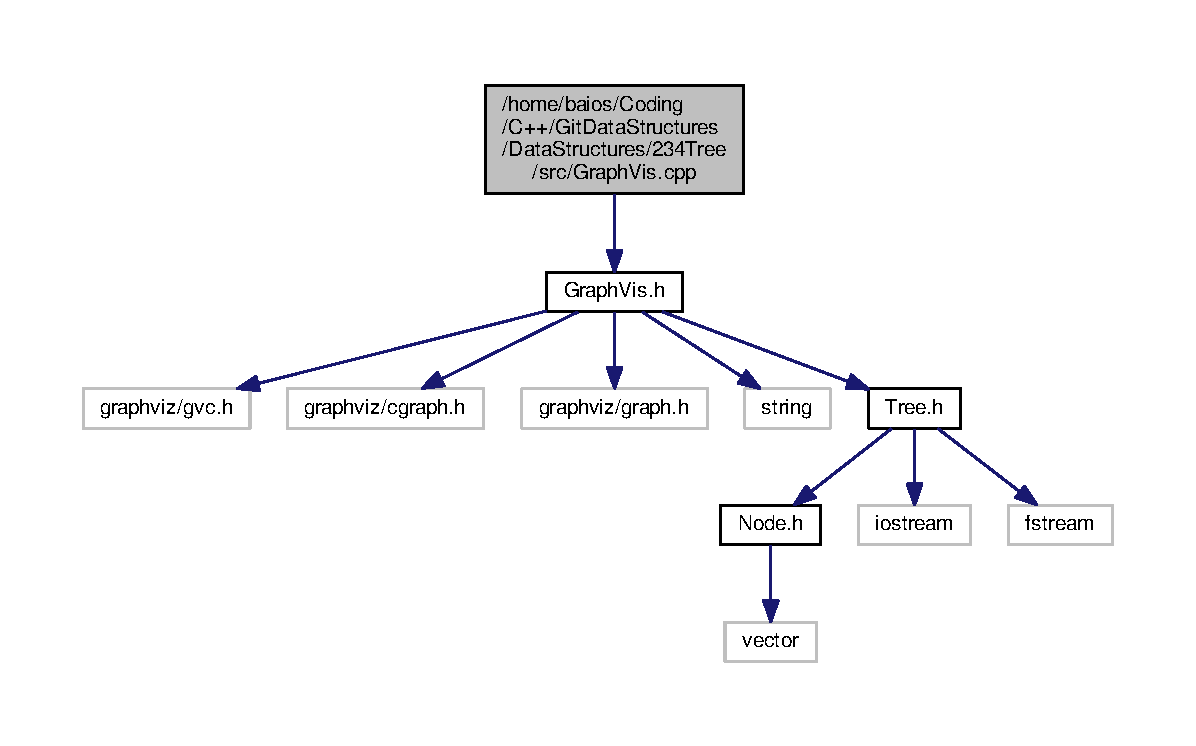
\includegraphics[width=350pt]{_graph_vis_8cpp__incl}
\end{center}
\end{figure}

\hypertarget{_interface_8cpp}{\section{/home/baios/\-Coding/\-C++/\-Git\-Data\-Structures/\-Data\-Structures/234\-Tree/src/\-Interface.cpp File Reference}
\label{_interface_8cpp}\index{/home/baios/\-Coding/\-C++/\-Git\-Data\-Structures/\-Data\-Structures/234\-Tree/src/\-Interface.\-cpp@{/home/baios/\-Coding/\-C++/\-Git\-Data\-Structures/\-Data\-Structures/234\-Tree/src/\-Interface.\-cpp}}
}
{\ttfamily \#include \char`\"{}Interface.\-h\char`\"{}}\\*
{\ttfamily \#include \char`\"{}Graph\-Vis.\-h\char`\"{}}\\*
{\ttfamily \#include $<$iostream$>$}\\*
Include dependency graph for Interface.\-cpp\-:
\nopagebreak
\begin{figure}[H]
\begin{center}
\leavevmode
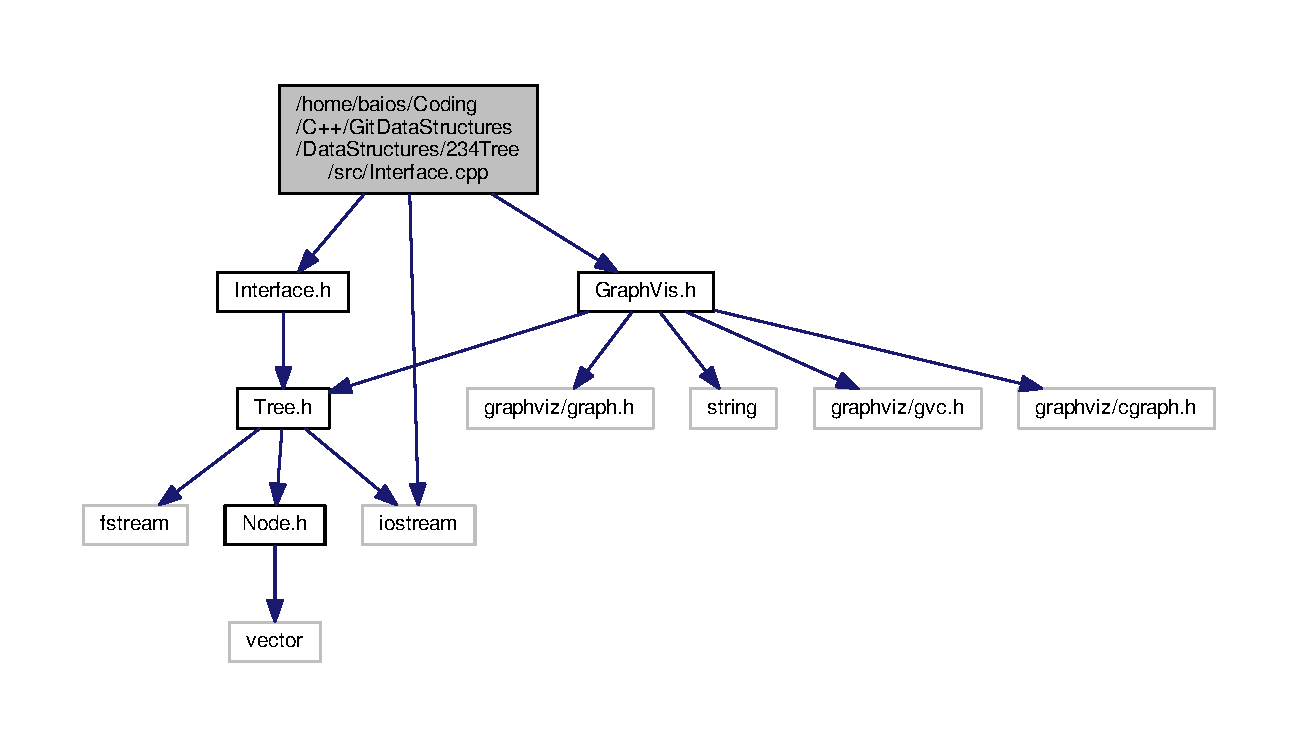
\includegraphics[width=350pt]{_interface_8cpp__incl}
\end{center}
\end{figure}

\hypertarget{main_8cpp}{\section{/home/baios/\-Desktop/\-Git\-Data\-Structures/\-Data\-Structures/\-Sorting\-And\-Searching/src/main.cpp File Reference}
\label{main_8cpp}\index{/home/baios/\-Desktop/\-Git\-Data\-Structures/\-Data\-Structures/\-Sorting\-And\-Searching/src/main.\-cpp@{/home/baios/\-Desktop/\-Git\-Data\-Structures/\-Data\-Structures/\-Sorting\-And\-Searching/src/main.\-cpp}}
}
{\ttfamily \#include \char`\"{}Sort\-\_\-\-N\-\_\-\-Search.\-h\char`\"{}}\\*
Include dependency graph for main.\-cpp\-:\nopagebreak
\begin{figure}[H]
\begin{center}
\leavevmode
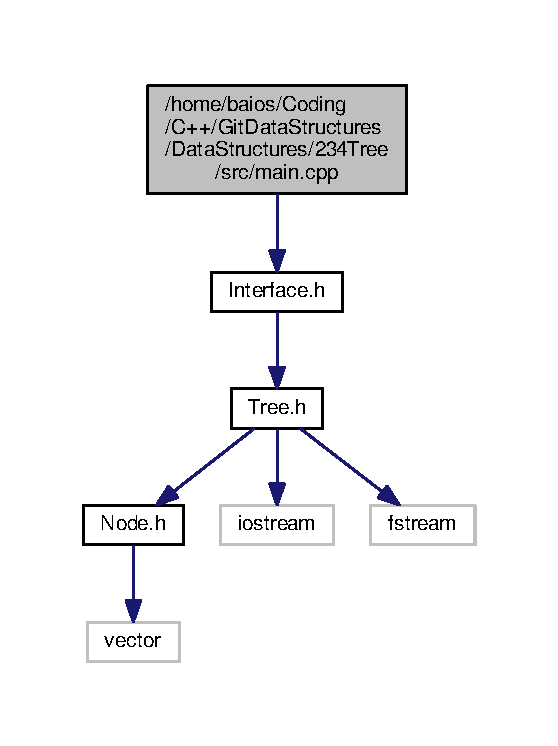
\includegraphics[width=350pt]{main_8cpp__incl}
\end{center}
\end{figure}
\subsection*{Functions}
\begin{DoxyCompactItemize}
\item 
int \hyperlink{main_8cpp_a3c04138a5bfe5d72780bb7e82a18e627}{main} (int argc, char $\ast$$\ast$argv)
\end{DoxyCompactItemize}


\subsection{Function Documentation}
\hypertarget{main_8cpp_a3c04138a5bfe5d72780bb7e82a18e627}{\index{main.\-cpp@{main.\-cpp}!main@{main}}
\index{main@{main}!main.cpp@{main.\-cpp}}
\subsubsection[{main}]{\setlength{\rightskip}{0pt plus 5cm}int main (
\begin{DoxyParamCaption}
\item[{int}]{argc, }
\item[{char $\ast$$\ast$}]{argv}
\end{DoxyParamCaption}
)}}\label{main_8cpp_a3c04138a5bfe5d72780bb7e82a18e627}

\begin{DoxyParams}{Parameters}
{\em Takes} & in an integer which represents the array size. \\
\hline
\end{DoxyParams}


Definition at line 33 of file main.\-cpp.



Here is the call graph for this function\-:\nopagebreak
\begin{figure}[H]
\begin{center}
\leavevmode
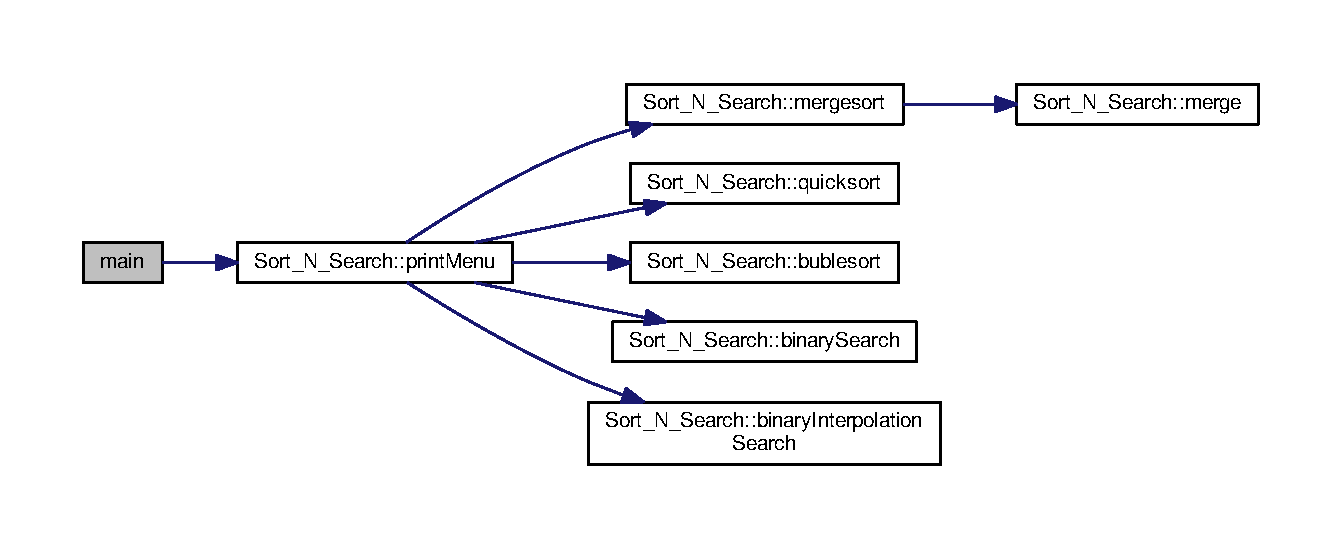
\includegraphics[width=350pt]{main_8cpp_a3c04138a5bfe5d72780bb7e82a18e627_cgraph}
\end{center}
\end{figure}



\hypertarget{_node_8cpp}{\section{/home/baios/\-Coding/\-C++/\-Git\-Data\-Structures/\-Data\-Structures/234\-Tree/src/\-Node.cpp File Reference}
\label{_node_8cpp}\index{/home/baios/\-Coding/\-C++/\-Git\-Data\-Structures/\-Data\-Structures/234\-Tree/src/\-Node.\-cpp@{/home/baios/\-Coding/\-C++/\-Git\-Data\-Structures/\-Data\-Structures/234\-Tree/src/\-Node.\-cpp}}
}
{\ttfamily \#include \char`\"{}Node.\-h\char`\"{}}\\*
Include dependency graph for Node.\-cpp\-:
\nopagebreak
\begin{figure}[H]
\begin{center}
\leavevmode
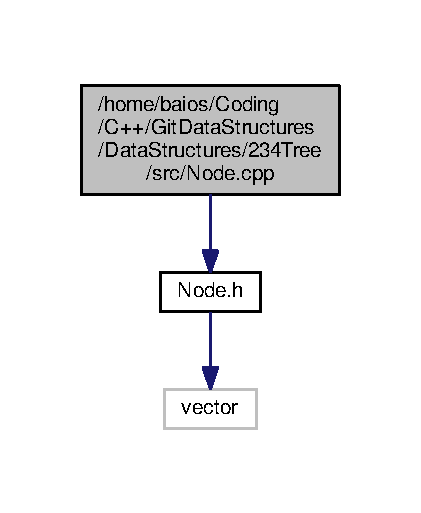
\includegraphics[width=202pt]{_node_8cpp__incl}
\end{center}
\end{figure}

\hypertarget{_tree_8cpp}{\section{/home/baios/\-Coding/\-C++/\-Git\-Data\-Structures/\-Data\-Structures/234\-Tree/src/\-Tree.cpp File Reference}
\label{_tree_8cpp}\index{/home/baios/\-Coding/\-C++/\-Git\-Data\-Structures/\-Data\-Structures/234\-Tree/src/\-Tree.\-cpp@{/home/baios/\-Coding/\-C++/\-Git\-Data\-Structures/\-Data\-Structures/234\-Tree/src/\-Tree.\-cpp}}
}
{\ttfamily \#include \char`\"{}Tree.\-h\char`\"{}}\\*
Include dependency graph for Tree.\-cpp\-:
\nopagebreak
\begin{figure}[H]
\begin{center}
\leavevmode
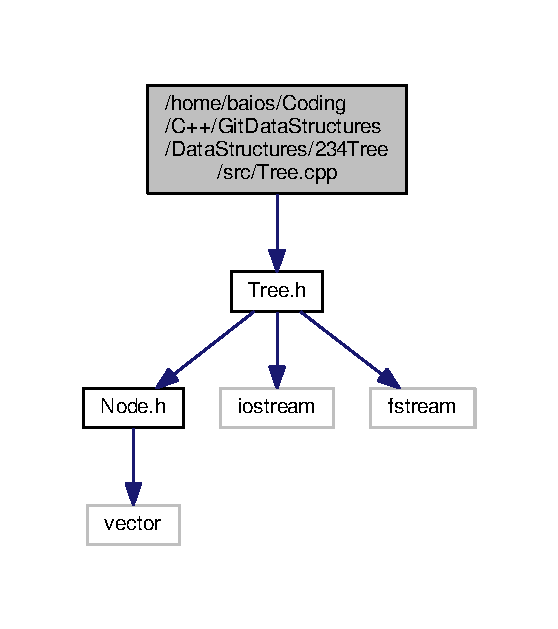
\includegraphics[width=268pt]{_tree_8cpp__incl}
\end{center}
\end{figure}

%--- End generated contents ---

% Index
\newpage
\phantomsection
\addcontentsline{toc}{chapter}{Index}
\printindex

\end{document}
